\chapter{Optical MIMO: Exploring the color dimension}
\label{chapter:mimoColor}
\thispagestyle{myheadings}
As seen in previous chapter, imaging receivers have the potential to to provide significant performance gains for a spatial MIMO OWC system. To incorporate these in portable devices, they must address challenges of being low powered, have fast sampling rates while incorporating optics, sensor and electronics in a small form factor.

This chapter explores the color dimension to establish an optical MIMO channel. It investigates color shift keying (CSK) as specified in IEEE 80.15.7 standard PHY  \rmnum{3}. The standard specifies a simplified linear system model for CSK. The human visual perception model is non--linear and needs to be considered while providing illumination. Thus a non--linear CSK model is investigated for different color band combinations. Luminous-signal-to-noise ratio metric is introduced to make fair performance comparisons between different modulation techniques operating at different average radiant flux, but same average luminous flux levels. Metameric modulation then further explores color dimension by using multiple sets of LEDs to transmit information over metamerically equivalent SPDs \cite{but12a}.

% -------------------------------------
% SECTION: IEEE 802.15.7
% -------------------------------------
\section{IEEE 802.15.7 - PHY\rmnum{3}}
\label{sec:ieeestd}
\graphicspath{{_MIMOColor/figures_csk/}}
LED based luminaires are energy efficient and are thus being widely adopted in indoor spaces to provide illumination. In order to dynamically control the rendered illumination spectrum, luminaires contain multiple elements of at least three colors of LEDs. Different rendered spectra, or spectral power distributions (SPDs), can be generated by mixing different ratios of radiant flux emitted from the multiple LEDs comprising a luminaire. Each resulting SPD realizes a different color mix to the human eye.

Any SPD within the visible range of electromagnetic spectrum can produce a stimulus when incident on the sensors of the human eye (rod and cones) and has a color associated with it. This color can also be represented by its intensity, hue and saturation. While intensity is a measure of the total power comprising the SPD, hue and saturation are subjective parameters analogous to mean and spread of the wavelengths comprising the SPD and are quantified by a chromaticity coordinate. The \textit{commission internationale de l'eclairage} (CIE) has specified the CIE 1931 XYZ color space (CIE-CS) that provides a mathematical model to represent the chromaticity of radiation in the visible range as a point in a 2-dimensional plane. Let a luminaire be comprised of three types of LEDs, namely LED$_{n}$; $n\in$ \text{\{i, j, k\}}. The chromaticity of each LED can be represented by a coordinate ($x_{n}$, $y_{n}$) on the CIE-CS. When different intensities of radiant flux emitted by three types of LEDs are combined, the chromaticity coordinate of the resultant SPD will lie inside the triangle formed by coordinates of the LEDs themselves.

\renewcommand{\arraystretch}{1.1}
\begin{table}[t]
\centering
\begin{tabular}{|c|c|c|c|c|}
\hline
\multirow{2}{*}{\textbf{CB$_{u}$}} & \textbf{Band} & \textbf{Center} & \multirow{2}{*}{\textbf{x}} & \multirow{2}{*}{\textbf{y}}\\
 & \textbf{(nm)} & \textbf{(nm)} & & \\
\hline
CB$_{0}$ & 380 - 478 & 429 & 0.169 & 0.007\\
\hline
CB$_{1}$ & 478 - 540 & 509 & 0.011 & 0.733\\
\hline
CB$_{2}$ & 540 - 588 & 564 & 0.402 & 0.597\\
\hline
CB$_{3}$ & 588 - 633 & 611 & 0.669 & 0.331\\
\hline
CB$_{4}$ & 633 - 679 & 656 & 0.729 & 0.271\\
\hline
CB$_{5}$ & 679 - 726 & 703 & 0.734 & 0.265\\
\hline
CB$_{6}$ & 726 - 780 & 753 & 0.734 & 0.265\\
\hline
\multicolumn{5}{c}{ }
\end{tabular}
\caption{Color bands.}
\label{tCB}
\end{table}
\renewcommand{\arraystretch}{1.0}

\begin{figure}[b]
\centering
		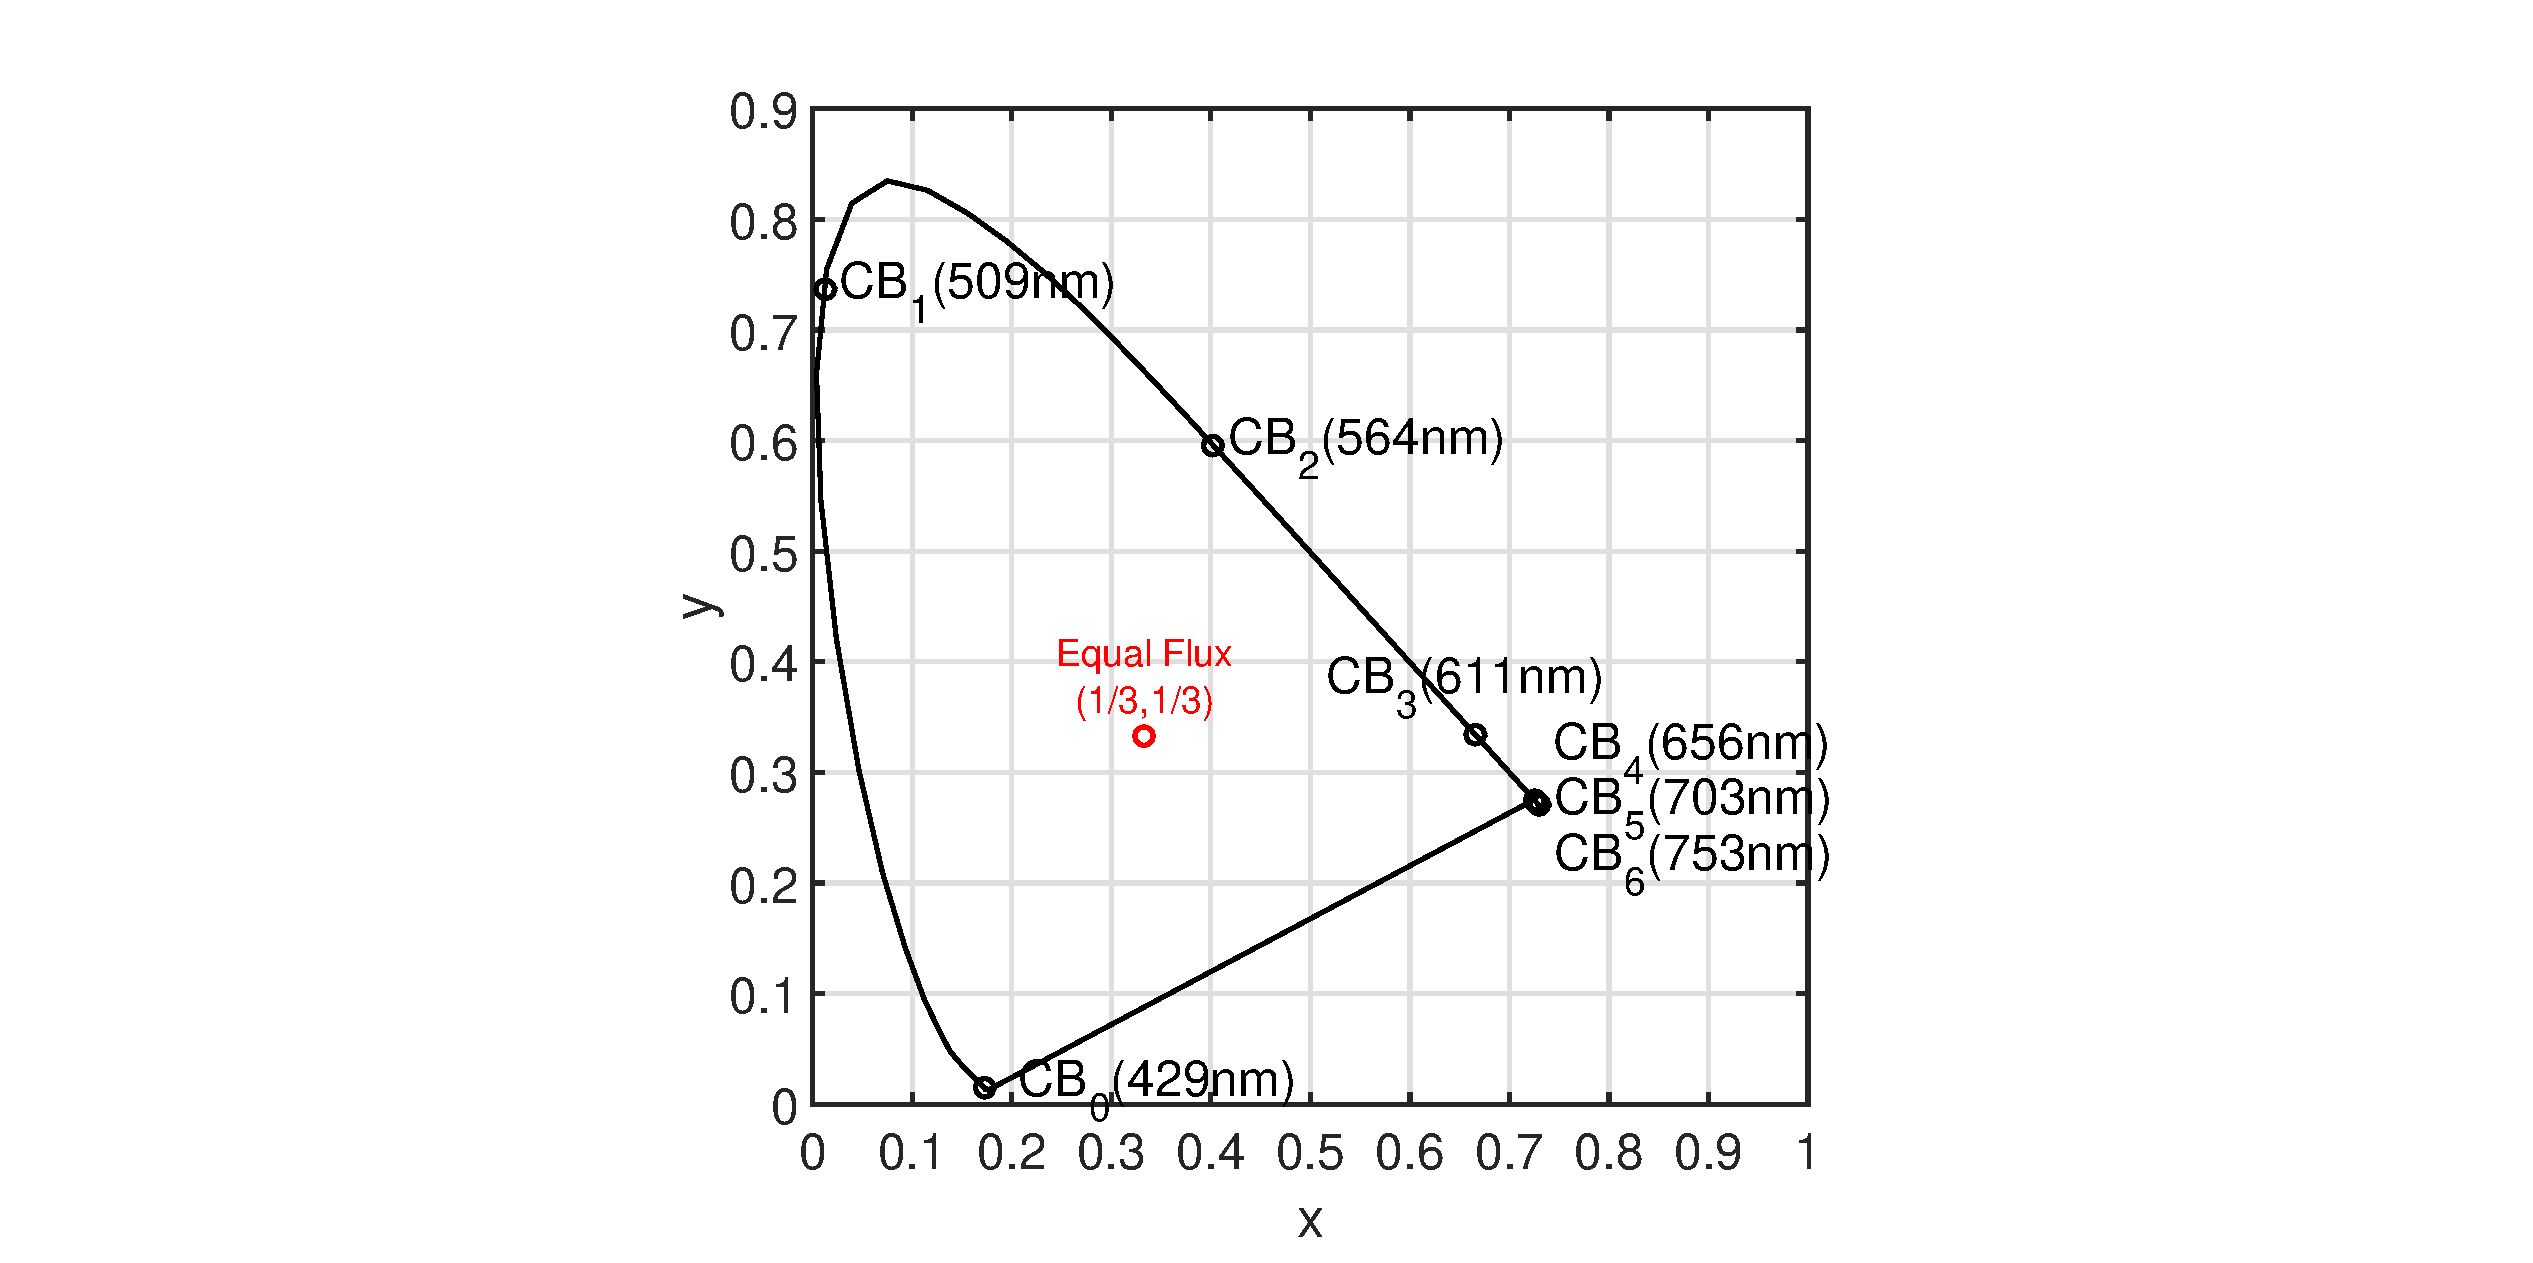
\includegraphics[trim={4.3in 0in 4.3in 0.5in}, clip=true, width=2.0in]{CBCcenters.eps}
	\caption{Color band centers on CIE-CS.}
	\label{figCBCcenters}
\end{figure}

CSK is a modulation technique in which information is transmitted through changes in chromaticity coordinates. This can be achieved by varying the intensities of LED$_{n}$ over time. To select sources for CSK implementation, the standard specifies 7 different color bands - CB$_{u}$; $0\leq u < 7$ by splicing the visible spectrum range into 7 contiguous segments as shown in Table \ref{tCB}. The center wavelength of each segment as represented on CIE-CS is illustrated in \figurename{ }\ref{figCBCcenters}. Note that even though center wavelengths of CB$_{4}$, CB$_{5}$ and CB$_{6}$ are 47 nm -- 50 nm apart, the distance between their chromaticity coordinates is very small. The CIE-CS is designed such that the SPD resulting from identical flux emitted by the three primary sources maps to coordinate (1/3, 1/3) which is shown in \figurename{ }\ref{figCBCcenters}. We can define a color sector on the CIE-CS as the region enclosed by a color band on the perimeter and coordinate (1/3, 1/3). Though not explicitly mentioned in the standard, it is assumed that SPD of each LED$_{n}$ must belong to a different color sector. To study the performance of CSK independent of specific LED characteristics, it is generally assumed that the chromaticity coordinate of an LED belonging to a color sector corresponds to the center wavelength of a color band CB$_{u}$ at the perimeter of the sector as illustrated in \figurename{ }\ref{figCBCcenters}.

\renewcommand{\arraystretch}{1.1}
\begin{table}[t]
\centering
\begin{tabular}{|c|c|c|c|}
\hline
Color band combination & \multicolumn{3}{c|}{Color band '$u$' for CBC$_{v}$} \\
\cline{2-4}
\textbf{CBC$_{v}$} & \textbf{Band i} & \textbf{Band j} & \textbf{Band k} \\
\hline
CBC$_{1}$ & 6 & 2 & 0 \\
\hline
CBC$_{2}$ & 6 & 1 & 0 \\
\hline
CBC$_{3}$ & 5 & 2 & 0 \\
\hline
CBC$_{4}$ & 5 & 1 & 0 \\
\hline
CBC$_{5}$ & 4 & 2 & 0 \\
\hline
CBC$_{6}$ & 4 & 1 & 0 \\
\hline
CBC$_{7}$ & 3 & 2 & 0 \\
\hline
CBC$_{8}$ & 3 & 1 & 0 \\
\hline
CBC$_{9}$ & 2 & 1 & 0 \\
\hline
\end{tabular}
\caption{Color bands combinations as specified by the standard.}
\label{tCBC}
\end{table}
\renewcommand{\arraystretch}{1.0}

\afterpage{%
\clearpage
\begin{landscape}% Landscape page
\renewcommand{\arraystretch}{1.1}
\begin{table}
\centering
\begin{tabular}{|c|c|c|c|}
\hline
\textbf{m} & \textbf{$M$ = 4} & \textbf{$M$ = 8} & \textbf{$M$ = 16} \\
\hline
0 & C$^{v}_{\text{j}}$ & (2C$_{4}$+C$_{5}$)/3 & C$^{v}_{\text{j}}$\\
1 & (C$^{v}_{\text{i}}$+C$^{v}_{\text{j}}$+C$^{v}_{\text{k}}$)/3 & (2C$_{a}$+C$_{b}$)/3; C$_{a}$=(C$_{b}$+C$_{3}$+C$_{5}$)/3; C$_{b}$=(C$_{4}$+C$_{5}$)/2 & (C$_{0}$+C$_{3}$+C$_{5}$)/3 \\
2 & C$^{v}_{\text{k}}$ & (2C$_{a}$+C$_{b}$)/3; C$_{a}$=(C$_{b}$+C$_{3}$+C$_{7}$)/3; C$_{b}$=(C$_{4}$+C$_{7}$)/2 & (C$_{3}$+C$_{6}$+C$_{10}$)/3 \\
3 & C$^{v}_{\text{i}}$ & (C$_{5}$+C$_{7}$)/2 & (2C$_{0}$+C$_{9}$)/3 \\
\cline{2-2}
4 & & C$^{v}_{\text{j}}$ & (C$_{0}$+2C$_{8}$)/3 \\
5 & & C$^{v}_{\text{k}}$ & (2C$_{0}$+C$_{8}$)/3 \\
6 & & (2C$_{4}$+C$_{7}$)/3 & (C$_{0}$+C$_{8}$+C$_{9}$)/3 \\
7 & & C$^{v}_{\text{i}}$ & (C$_{4}$+C$_{5}$+C$_{6}$)/3 \\
\cline{3-3}
8 & & & C$^{v}_{\text{i}}$ \\
9 & & & C$^{v}_{\text{k}}$ \\
10 & & & (C$_{0}$+2C$_{9}$)/3 \\
11 & & & (C$_{9}$+C$_{10}$+C$_{15}$)/3 \\
12 & & & (2C$_{8}$+C$_{9}$)/3 \\
13 & & & (C$_{4}$+C$_{8}$+C$_{12}$)/3 \\
14 & & & (C$_{6}$+C$_{12}$+C$_{15}$)/3 \\
15 & & & (C$_{8}$+2C$_{9}$)/3 \\
\hline
\end{tabular}
\caption{Design rules to compute constellation points for $M$-ary CSK. Each row computes C$_{m}$, the chromaticity coordinate for m$^{th}$ codeword for any given CBC$_{v}$. C$^{v}_{n}$ is the chromaticity coordinate of color band $n\in$ \{i, j, k\} belonging to CBC$_{v}$.}
\label{tMCSK}
\end{table}
\renewcommand{\arraystretch}{1.0}
\end{landscape}
\clearpage% Flush page
}

To implement CSK using 3 types of LEDs, the standard defines different sets of 3 color bands and calls each set a color band combination (CBC). The 3 different types of LEDs forming a CBC are ordered in a descending manner based on the center wavelength of the color band they belong to and each such band is called `band i', `band j' and `band k' respectively. 9 such CBC$_{v}$; $1\leq v\leq 9$ are defined in the standard and are outlined in Table \ref{tCBC}. For the rest of this article, generalized notation CB$^{v}_{n}$ will be used to indicate color band of type $n\in$ \text{\{i, j, k\}} belonging to CBC$_{v}$. Thus in Table \ref{tCBC}, the cell representing row for CBC$_{v}$ and column for band $n$ provides index $u$ for the color band represented by notation CB$^{v}_{n}$. Using this notation CB$^{1}_{\text{i}}$ $\equiv$ CB$_{6}$ while CB$^{2}_{\text{j}}$ $\equiv$ CB$_{1}$ and so on.

For an $M$-ary CSK using CBC$_{v}$, the design rules to compute the $M$ different constellation points are provided in the standard and their values are outlined in \cite{cskxy}. Let C$^{v}_{n}$ $\equiv$ (x$^{v}_{n}$, y$^{v}_{n}$) be chromaticity coordinate corresponding to CB$^{v}_{n}$. Let C$_{m}$ $\equiv$ ($x_{m}$, $y_{m}$); $0\leq m <$ $M$ be chromaticity coordinate corresponding to m$^{th}$ codeword. Then Table 3 outlines the design rules for computing the constellation points. C$^{v}_{n}$ can be looked up from Table \ref{tCBC} and Table \ref{tCB}. Using these values, remaining C$_{m}$ can then be computed using rules from Table \ref{tMCSK}. Normalized constellation design rules for $M$-ary CSK are illustrated in \figurename{ }\ref{figConst}. Points I, J and K represent normalized coordinates for the $n$ color bands comprising a CBC. 

\afterpage{%
\clearpage
\begin{landscape}% Landscape page
\begin{figure}[t]
	\centering
		\begin{subfigure}{0.46\textwidth}
		\centering
			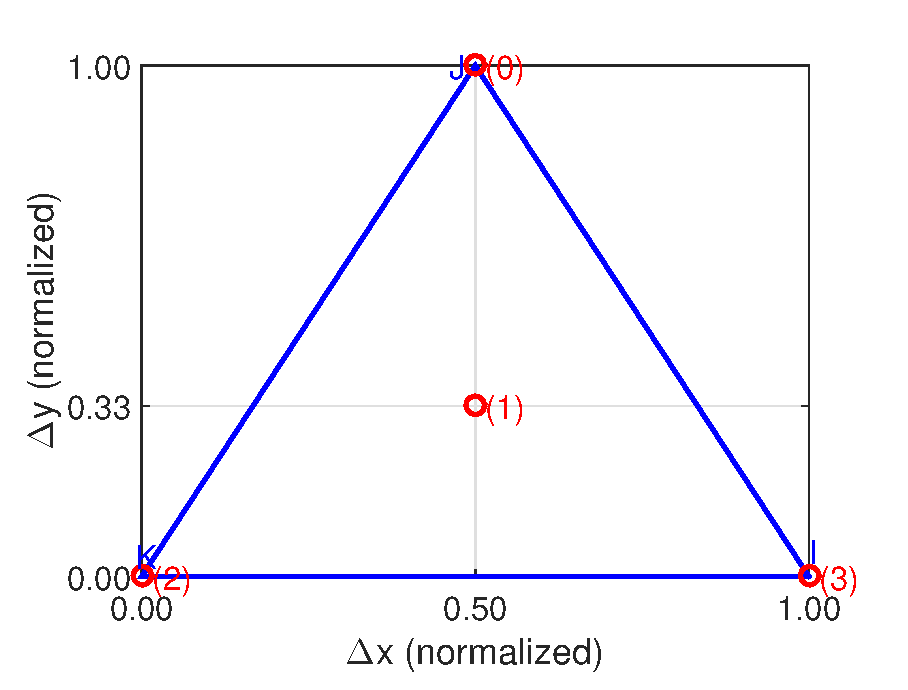
\includegraphics[trim={0.05in 0.0in 0.25in 0.2in}, clip=true, width=\textwidth]{CBCrules4.eps}
			\caption{4-CSK}
			\label{fig4Const}
		\end{subfigure}
		\hfill
		\begin{subfigure}{0.46\textwidth}
		\centering
			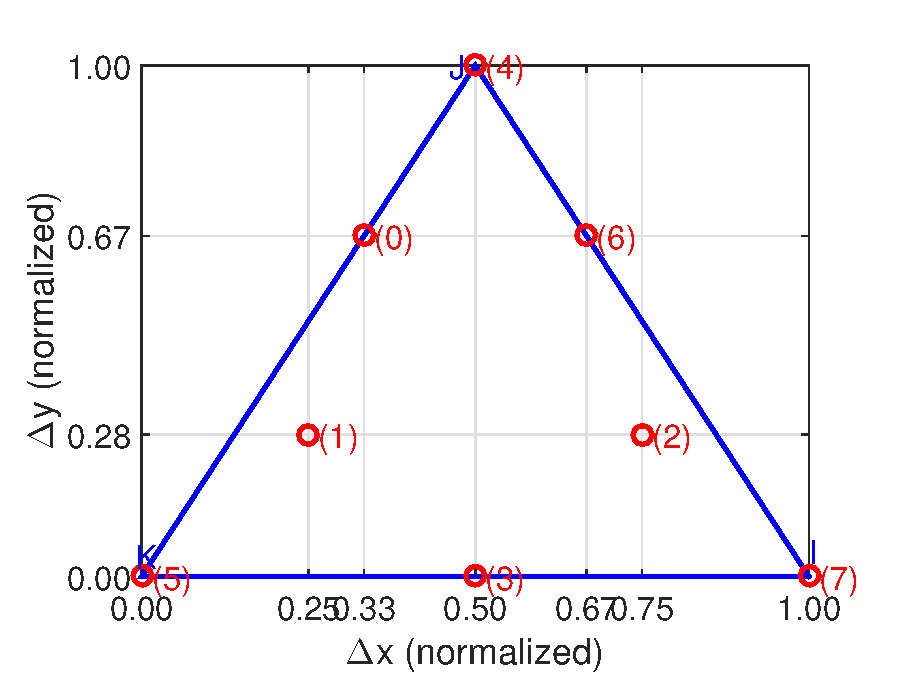
\includegraphics[trim={0.05in 0.0in 0.25in 0.2in}, clip=true, width=\textwidth]{CBCrules8.eps}
			\caption{8-CSK}
			\label{fig8Const}
		\end{subfigure}
		\hfill
		\begin{subfigure}{0.46\textwidth}
		\centering
			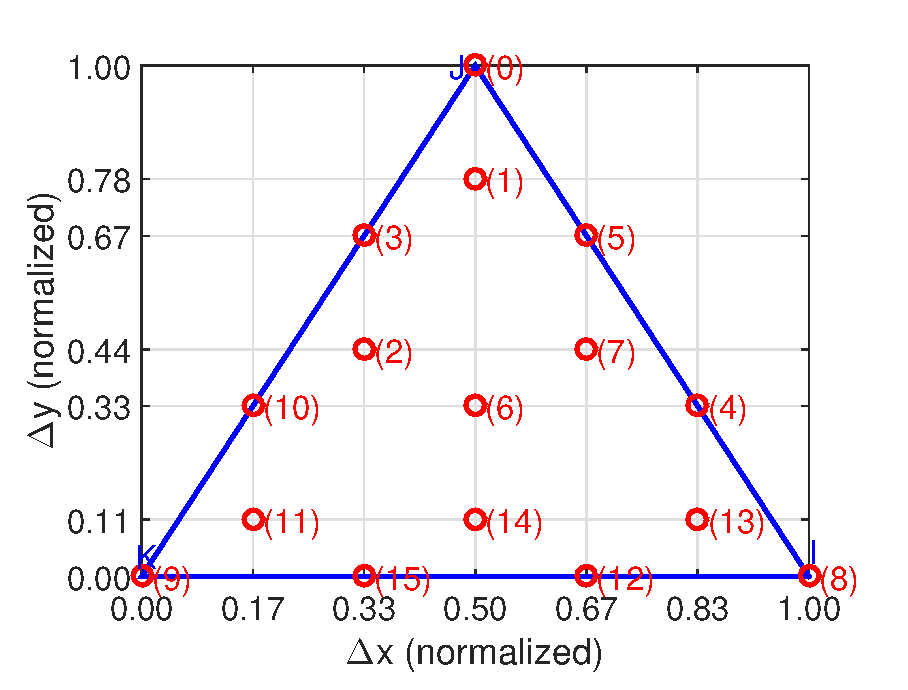
\includegraphics[trim={0.05in 0.0in 0.25in 0.2in}, clip=true, width=\textwidth]{CBCrules16.eps}
			\caption{16-CSK}
			\label{fig16Const}
		\end{subfigure}
	\caption{$M$-ary CSK (normalized) constellation design rules.}
	\label{figConst}
\end{figure}
\end{landscape}
\clearpage% Flush page
}

%\afterpage{%
%\clearpage
%\begin{landscape}% Landscape page
%
%\end{landscape}
%\clearpage% Flush page
%}
CSK is implemented in conjunction with IM/DD over the optical channel. This channel can be modeled as a linear time invariant system with additive white Gaussian noise (AWGN) and mathematically represented as in Eq.(\ref{eqCHNL})

\begin{equation}
	\vm{Y} = \vm{H}\vm{X} + \vm{W}
	\label{eqCHNL}
\end{equation}
where \vm{X} is an $n_{\text{tx}}$ dimensional vector containing transmit optical powers for each band $n$, \vm{H} is a $n_{\text{rx}}\times n_{\text{tx}}$ dimensional channel matrix, \vm{W} is a $n_{\text{rx}}$ dimensional noise vector and \vm{Y} is an $n_{\text{rx}}$ dimensional receive vector. Channel matrix \vm{H} includes the responsivities of the receive elements.

In $M$-ary CSK, $n_{\text{tx}}=3$ types of LEDs are used to generate $M$ different SPDs corresponding to $M$ different chromaticity coordinates. Each chromaticity coordinate represents a codeword that encodes lo $^{ }_{2}$($M$) bits. In order to transmit information, the luminaire irradiates an SPD corresponding to the desired transmit codeword. The clock rate at the luminaire is of the order of tens of MHz. This rate is much higher than which can be perceived by human eye as flicker. In addition, the CSK signaling chain can include a scrambler that ensures data and thus codewords are pseudo-randomly distributed thus mitigating color flicker.

At the receiving elements, each SPD produces a different electrical response signal. The signal output from each receiving element is corrupted by shot noise of variance $\sigma^{2}_{sh}$ due to ambient light and thermal noise of variance $\sigma^{2}_{th}$ due to trans-impedance amplifier as shown in Eq.(\ref{eqNOISE})

\begin{equation}
	\begin{aligned}
	\sigma^{2}_{sh} &= 2q<i>B\\
	\sigma^{2}_{th} &= \frac{4k_{B}TB}{R_{f}}
\end{aligned}
\label{eqNOISE}
\end{equation}
where $<i>$ is average current generated in the photodiode due incident ambient light, $q$ is charge of an electron, $k_{B}$ is Boltzmann's constant, $T$ is the temperature in Kelvin and $R_{f}$ is the amplifier feedback resistance and B is the channel bandwidth. The signal-to-noise ratio (SNR) can then be defined as in Eq.(\ref{eqSNR})

\begin{equation}
	\text{SNR} \triangleq \frac{\text{Tr}\{\vm{H}\vm{X}\vm{X}^{*}\vm{H}^{*}\}}{\sigma^{2}_{nt}}
	\label{eqSNR}
\end{equation}
where Tr$\{.\}$ is the matrix trace operator, $^{*}$ indicates transpose and $\sigma^{2}_{nt}=\sigma^{2}_{sh}+\sigma^{2}_{th}$ is the total noise variance. SNR in decibel is then computed as 10log$^{ }_{10}$(SNR).

Having received vector \vm{Y}, least squares estimate of transmitted vector ($\hat{\vm{X}}$) can be made by Eq.(\ref{eqXHAT}).
\begin{equation}
	\hat{\vm{X}} = (\vm{H}^{*}\vm{H})^{-1}\vm{H}^{*}\vm{Y}
	\label{eqXHAT}
\end{equation}

After estimating vector $\hat{\vm{X}}$, an estimate of transmitted chromaticity coordinates can be made and transmitted information can then be decoded. The process of transforming chromaticity coordinates to optical power and vice-versa gives rise to two different system models as described in further sections.


% -------------------------------------
% SECTION: CSK
% -------------------------------------
\section{Color shift keying}
\label{sec:csk}
\graphicspath{{_MIMOColor/figures_csk/}}

\subsection{CSK system outline}
\label{subsec:cskOutline}
CSK is implemented in conjunction with IM/DD over the optical channel. This channel can be modeled as a linear time invariant system with AWGN and mathematically represented as in Eq.(\ref{eqCHNL})

\begin{equation}
	\vm{Y} = \vm{H}\vm{X} + \vm{W}
	\label{eqCHNL}
\end{equation}
where \vm{X} is an $N_{\text{tx}}$ dimensional vector containing transmit optical powers for each band $n$, \vm{H} is a $N_{\text{rx}}\times N_{\text{tx}}$ dimensional channel matrix, \vm{W} is a $N_{\text{rx}}$ dimensional noise vector and \vm{Y} is an $N_{\text{rx}}$ dimensional receive vector. Channel matrix \vm{H} includes the responsivities of the receive elements.

In $M$-ary CSK, $N_{\text{tx}}=3$ types of LEDs are used to generate $M$ different SPDs corresponding to $M$ different chromaticity coordinates. Each chromaticity coordinate represents a codeword that encodes log$^{ }_{2}$($M$) bits. In order to transmit information, the luminaire irradiates an SPD corresponding to the desired transmit codeword. The clock rate at the luminaire is of the order of tens of MHz. This rate is much higher than which can be perceived by human eye as flicker. In addition, the CSK signaling chain can include a scrambler that ensures data and thus codewords are pseudo-randomly distributed thus mitigating color flicker.

At the receiving elements, each SPD produces a different electrical response signal. The signal output from each receiving element is corrupted by shot noise of variance $\sigma^{2}_{\text{sh}}$ due to ambient light and thermal noise of variance $\sigma^{2}_{\text{th}}$ due to trans-impedance amplifier as shown in Eq.(\ref{eqNOISE})

\begin{equation}
	\begin{aligned}
	\sigma^{2}_{\text{sh}} &= 2q<i>B\\
	\sigma^{2}_{\text{th}} &= \frac{4k_{B}TB}{R_{f}}
\end{aligned}
\label{eqNOISE}
\end{equation}
where $<i>$ is average current generated in the photodiode due incident ambient light, $q$ is charge of an electron, $k_{B}$ is Boltzmann's constant, $T$ is the temperature in Kelvin and $R_{f}$ is the amplifier feedback resistance and B is the channel bandwidth. The signal-to-noise ratio (SNR) can then be defined as in Eq.(\ref{eqSNR})

\begin{equation}
	\text{SNR} \triangleq \frac{\text{Tr}\{\vm{H}\vm{X}\vm{X}^{*}\vm{H}^{*}\}}{\sigma^{2}_{\text{nt}}}
	\label{eqSNR}
\end{equation}
where Tr$\{.\}$ is the matrix trace operator, $^{*}$ indicates transpose and $\sigma^{2}_{\text{nt}}=\sigma^{2}_{\text{sh}}+\sigma^{2}_{\text{th}}$ is the total noise variance. SNR in decibel is then computed as 10log$^{ }_{10}$(SNR).

Having received vector \vm{Y}, least squares estimate of transmitted vector ($\hat{\vm{X}}$) can be made by Eq.(\ref{eqXHAT}).
\begin{equation}
	\hat{\vm{X}} = (\vm{H}^{*}\vm{H})^{-1}\vm{H}^{*}\vm{Y}
	\label{eqXHAT}
\end{equation}

After estimating vector $\hat{\vm{X}}$, an estimate of transmitted chromaticity coordinates can be made and transmitted information can then be decoded. The process of transforming chromaticity coordinates to optical power and vice-versa gives rise to two different system models as described in further sections.

\subsection{Linear system model}
\label{subsec:cskLinear}
The linear CSK model treats the CIE-CS as a linear space to analyze CSK performance. This implies the inherent assumption that when irradiance from multiple transmitting elements is combined, the chromaticity coordinates of the resulting SPD is a linear combination of the chromaticity coordinates of the SPDs of individual transmitting elements. If P$_{n}$; $n\in$ \{i, j, k\} is the normalized radiant flux at the transmit or receive device associated with band $n$, Eq.(\ref{eqLIN}) below taken from the standard provides the implied mathematical relationships between chromaticity coordinates of all bands and that of resultant SPD.

\begin{equation}
	\begin{aligned}
	x_{\text{p}} &= \text{P}_{\text{i}}x_{\text{i}} + \text{P}_{\text{j}}x_{\text{j}} + \text{P}_{\text{k}}x_{\text{k}}\\
	y_{\text{p}} &= \text{P}_{\text{i}}y_{\text{i}} + \text{P}_{\text{j}}y_{\text{j}} + \text{P}_{\text{k}}y_{\text{k}}\\
	1 &= \text{P}_{\text{i}} + \text{P}_{\text{j}} + \text{P}_{\text{k}}
\end{aligned}
\label{eqLIN}
\end{equation}

%\afterpage{%
%\clearpage
%\begin{landscape}% Landscape page
\begin{figure}[!t]
	\centering
		%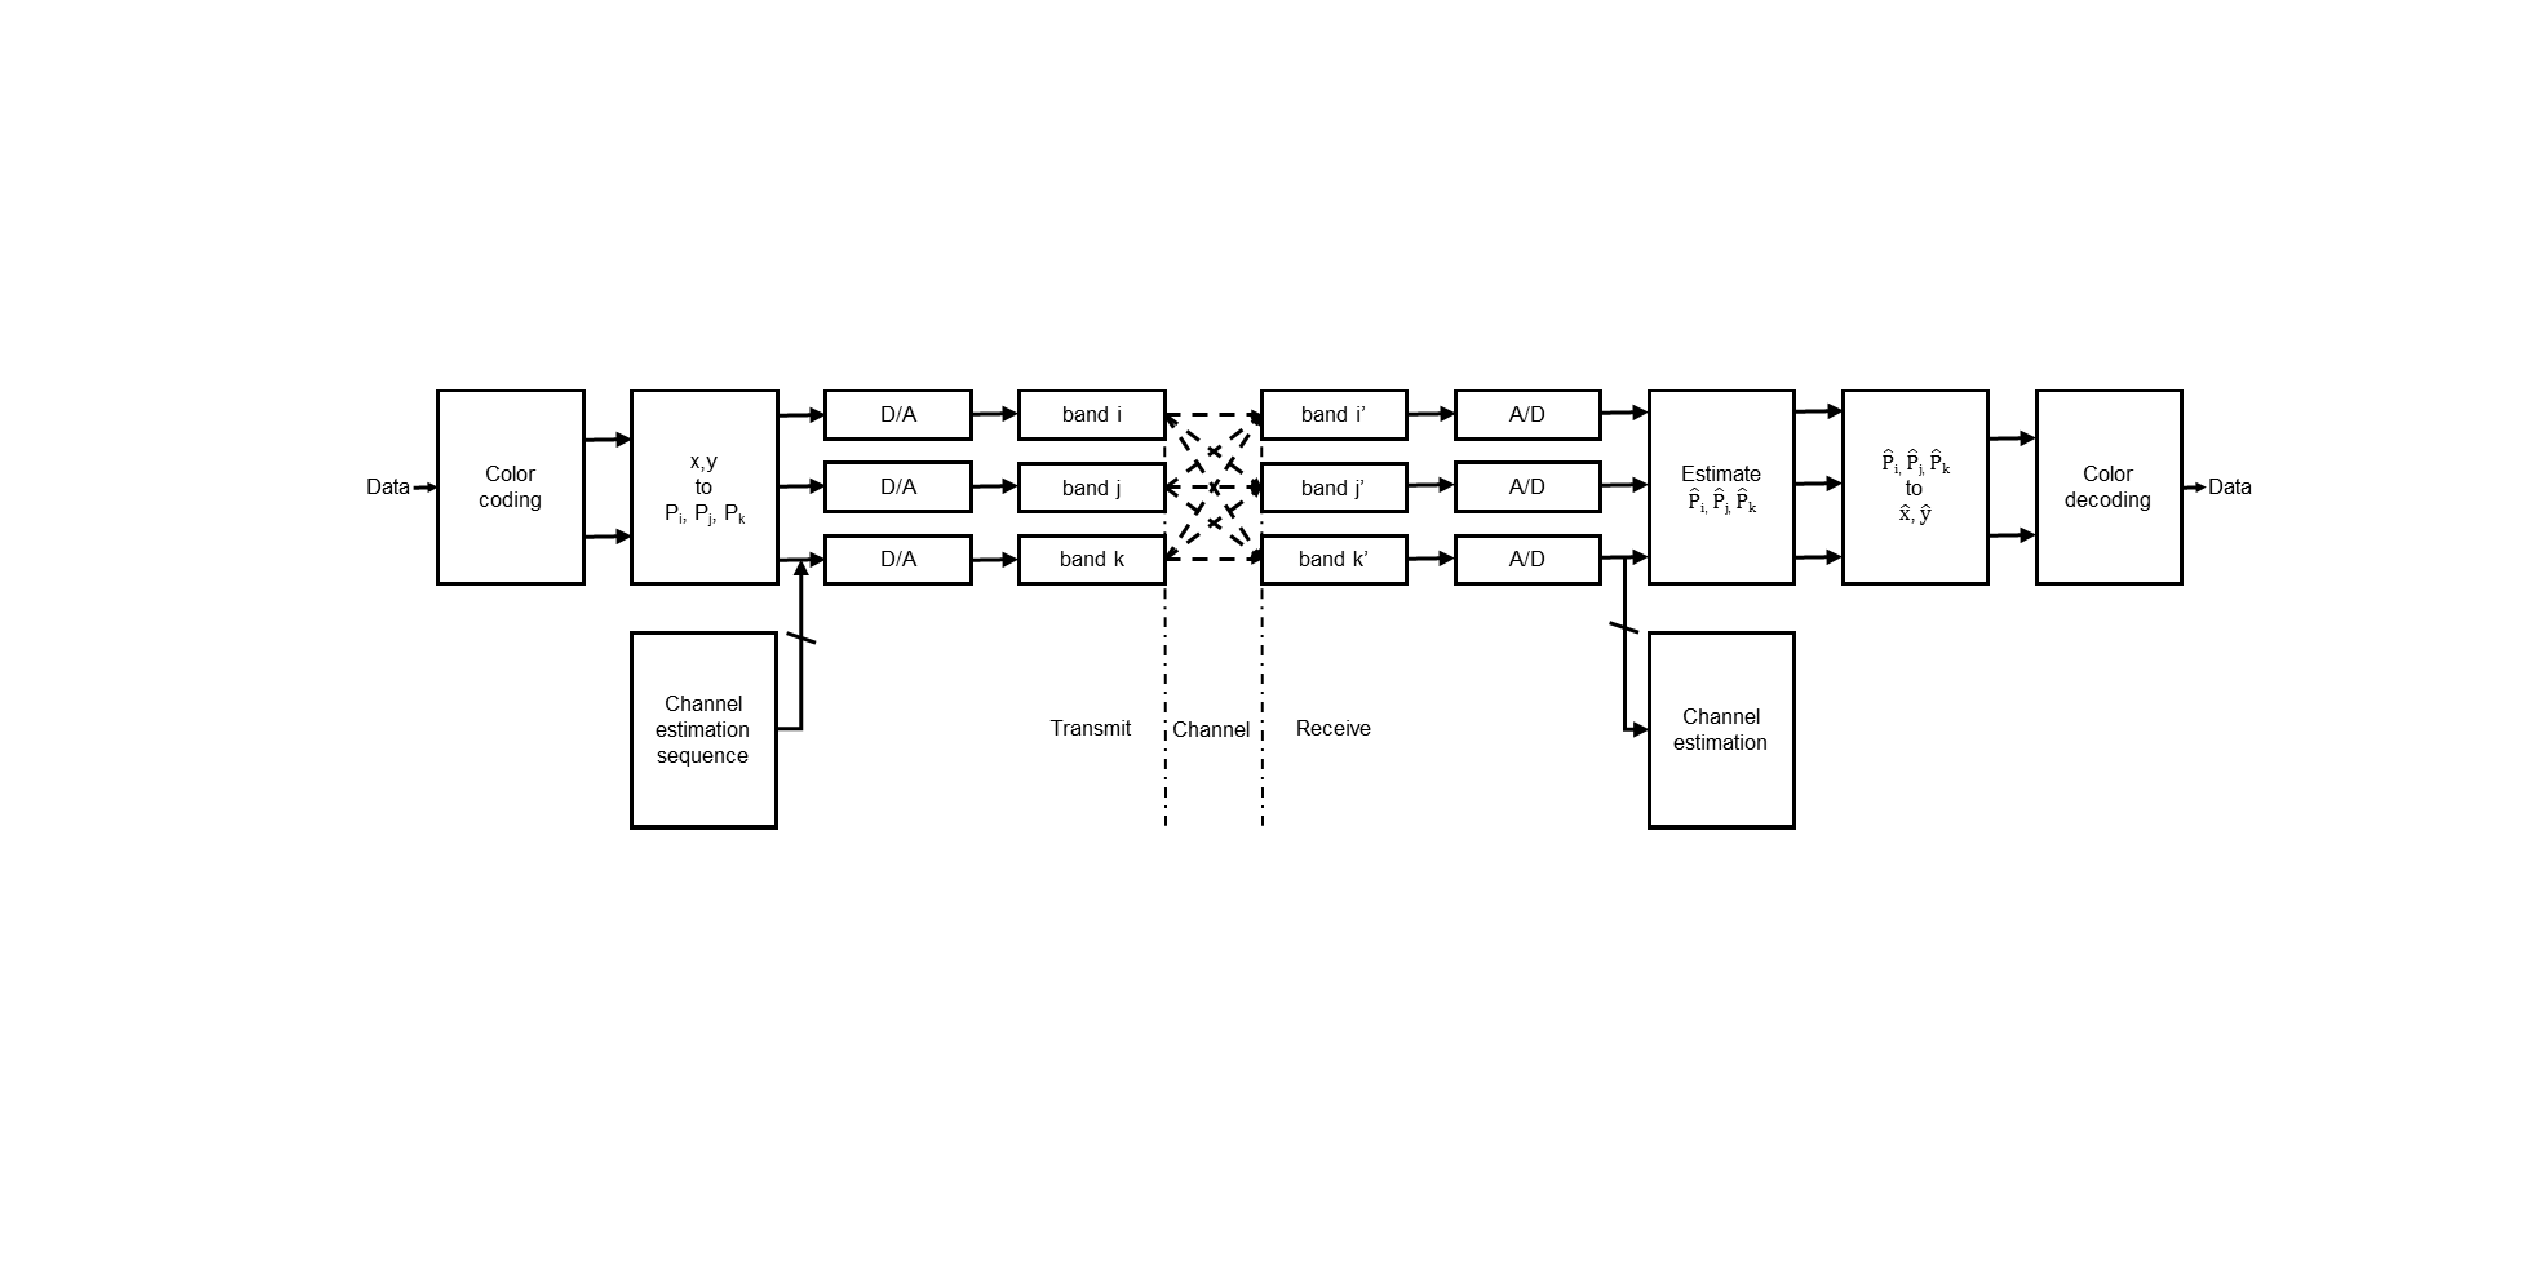
\includegraphics[trim={2.34in 2.78in 1.76in 2.47in}, clip=true, width=5.25in]{CSKBlockDiagram_1.eps}
		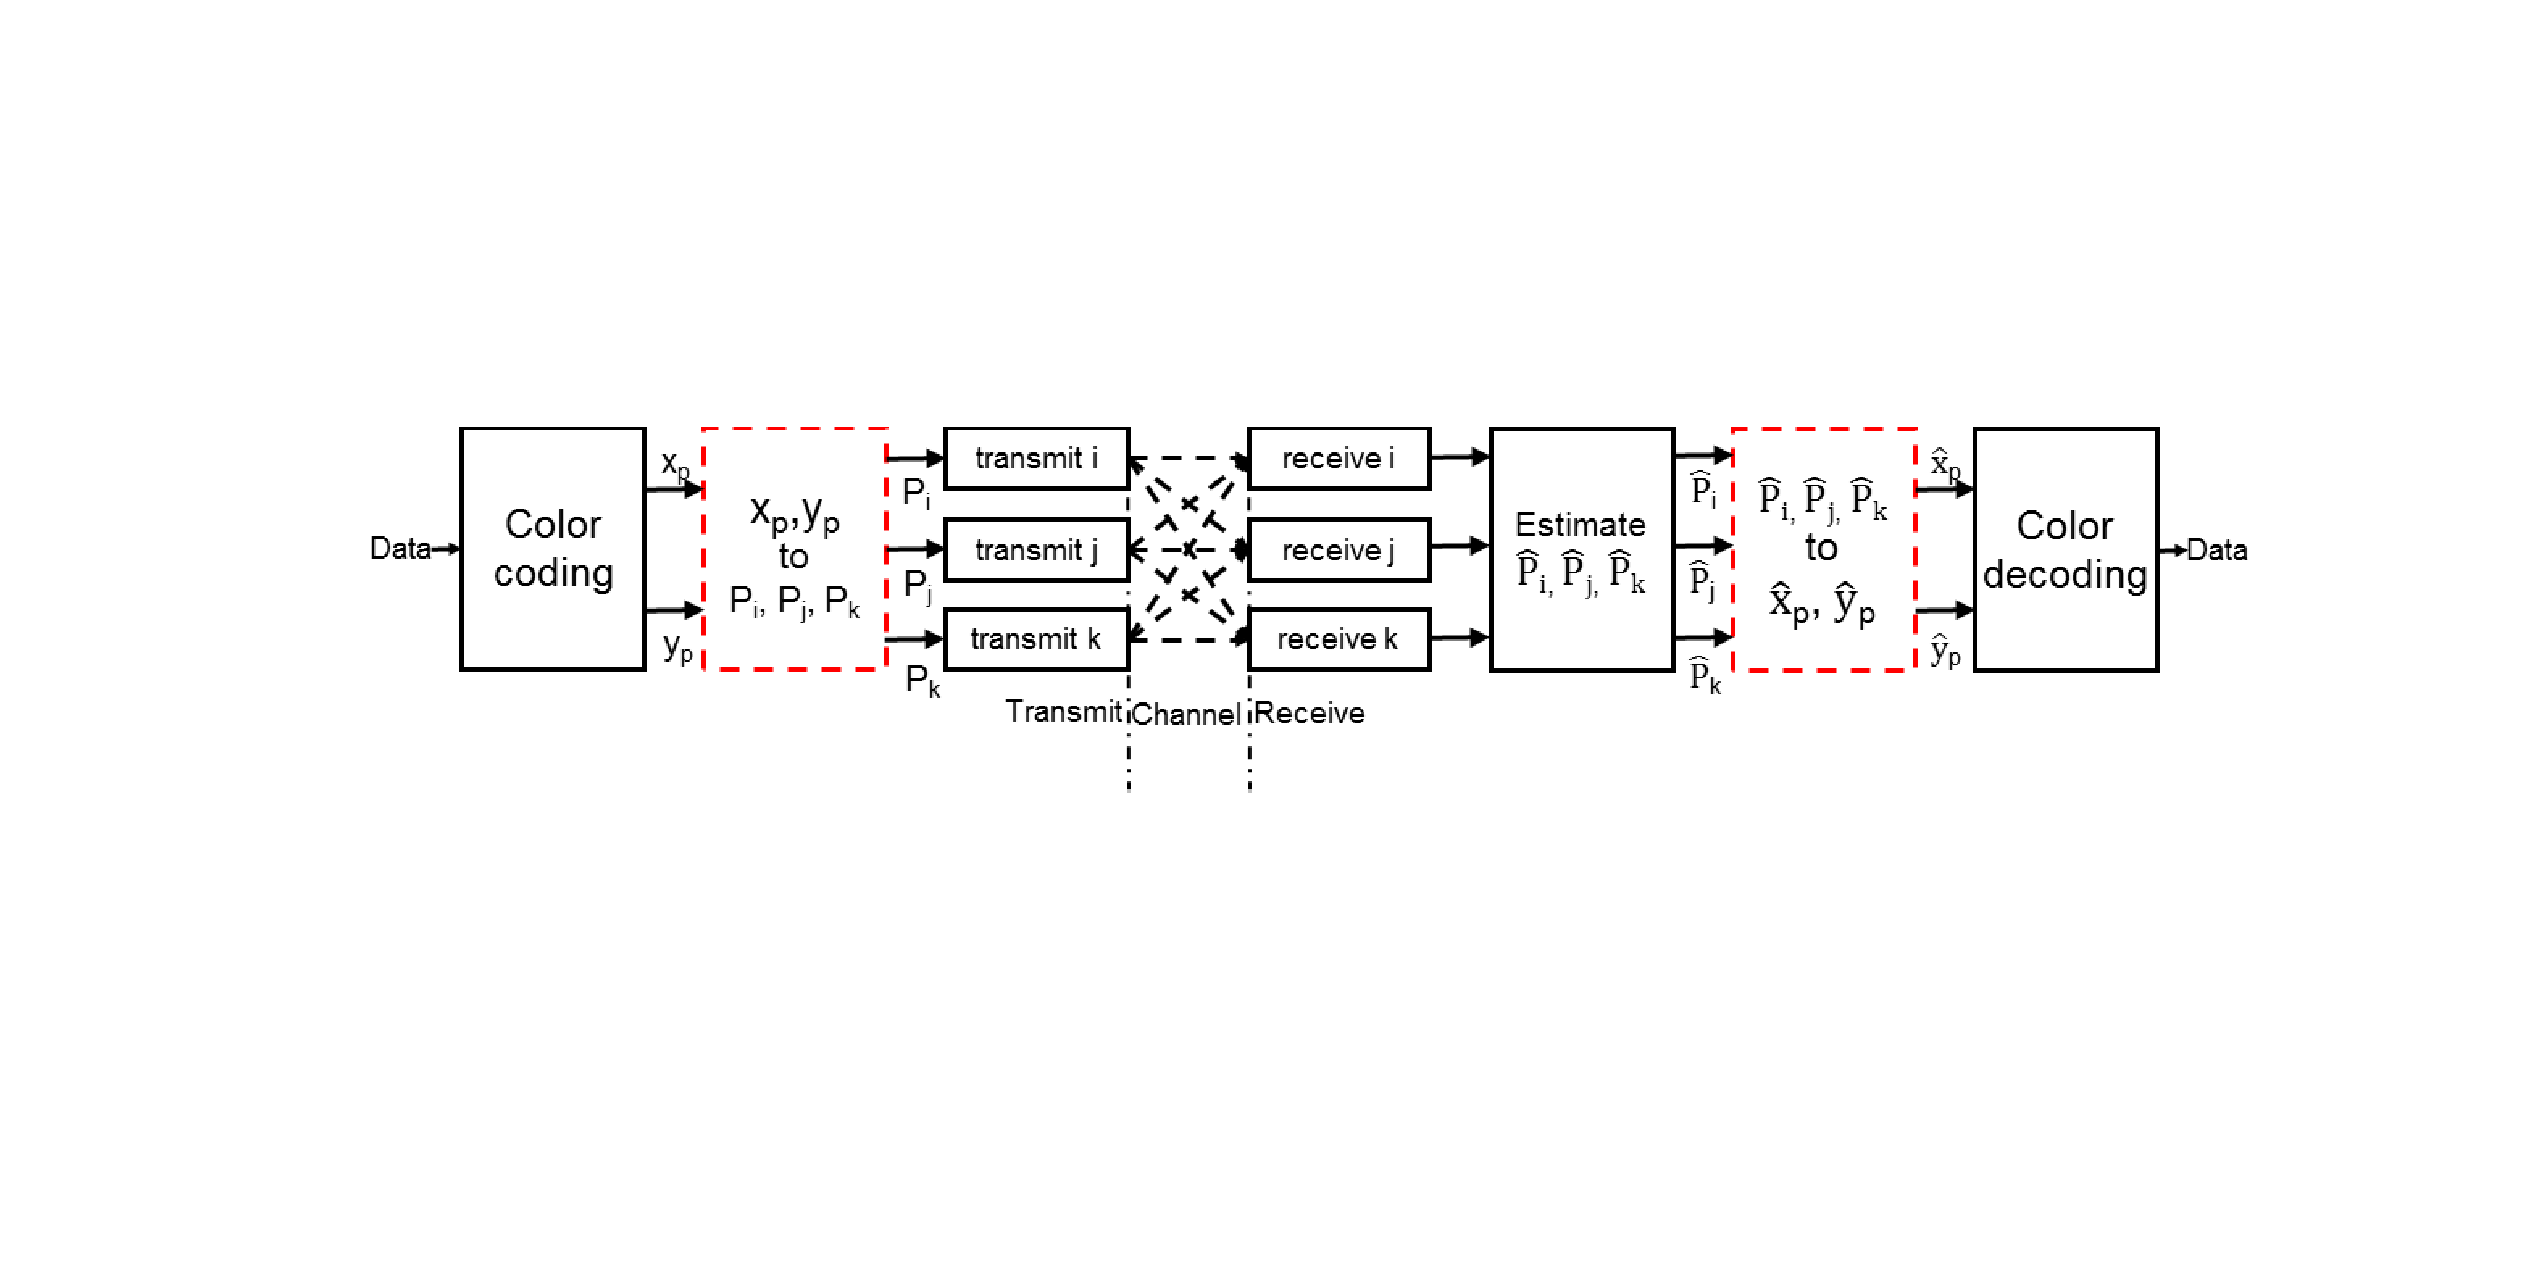
\includegraphics[trim={2.34in 2.78in 1.76in 2.47in}, clip=true, width=6in]{CSKBlockDiagram.eps}
	\caption{CSK signal chain block diagram}
	\label{figCSKBD}
\end{figure}
 %Implementation of red dashed blocks differentiates the linear and the non-linear system models.
%\end{landscape}
%\clearpage% Flush page
%}

A block diagram of the CSK signaling chain is shown in \figurename{ }\ref{figCSKBD}. At the transmitting element, the encoded information bit--stream is mapped to chromaticity coordinates ($x_{\text{p}}$, $y_{\text{p}}$) as computed from Table \ref{tMCSK}. Using Eq.(\ref{eqLIN}), normalized P$_{n}$ values are computed which are then scaled to achieve a user requested illumination target and thus transmit irradiance. A vector of scaled P$_{n}$ values then forms the transmit vector \vm{X}. Without loss of generality, unity E/O conversion at transmitter and unity responsivity (O/E conversion) at the receiver is assumed. Receiving element for band $n$ senses the incident flux and generates an electrical signal proportional to it. AWGN as computed from Eq.\eqref{eqNOISE} is then added to each band $n$ in the form of vector \vm{W}. The receiver output in presence of noise is represented by \vm{Y}. With the knowledge of the channel state and the receiver output, a least squares estimate of transmit vector $\hat{\vm{X}}$ is made using Eq.\eqref{eqXHAT}. Each element of $\hat{\vm{X}}$ then provides the estimates of transmitted flux represented by $\hat{\text{P}}_{n}$. Using these values, ($\hat{x}_{\text{p}}, \hat{y}_{\text{p}}$) are estimated using Eq.\eqref{eqLIN}. Nearest neighbor decoder then estimates the transmitted coordinate and recovers the transmitted information. Thus for the linear system model, Eq.\eqref{eqLIN} represents the ($x_{\text{p}}$, $y_{\text{p}}$) $\rightarrow  \text{P}_{n}$ and $\hat{\text{P}}_{n}\rightarrow$ ($\hat{x}_{\text{p}}$, $\hat{y}_{\text{p}}$) transformations for the red dashed blocks of \figurename{ }\ref{figCSKBD}.
%In this case the channel matrix \vm{H} is $N_{\text{rx}}\times N_{\text{tx}}$ dimensional identity matrix ($N_{\text{rx}}=N_{\text{tx}} = 3$).

Monte-carlo simulations are performed to compute performance of $M$-ary CSK under the linear model for all CBC$_{v}$ and \figurename{ }\ref{figBERvsSNR} shows the results. Performance of all CBCs is similar except CBC$_{7}$ and CBC$_{9}$ which perform slightly worse, but only by a margin of about 0.6 dB. This performance is as expected. As seen from Table \ref{tCBC}, CBC$_{7}$ is composed of CB$_{3}$, CB$_{2}$ and CB$_{0}$ whereas and CBC$_{9}$ is composed of CB$_{2}$, CB$_{1}$ and CB$_{0}$. Thus from values in Table \ref{tCB} and \figurename{ }\ref{figCBCcenters}, it can be seen that constellation points for other CBCs are the most spread out and have the large minimum distance between constellation points where as that for CBC$_{7}$ and CBC$_{9}$ have the shorter spread and have the smaller minimum distance between constellation points. SNR of at least 15 dB, 20 dB and 25 dB are needed to achieve a target minimum bit error rate (BER) of $10^{-3}$ under the linear model for $M$ = 4, 8 and 16 CSK respectively.

%\afterpage{%
%\clearpage
%\begin{landscape}% Landscape page
\begin{figure}[H]
	\centering
		\begin{subfigure}{\textwidth}
		\centering
			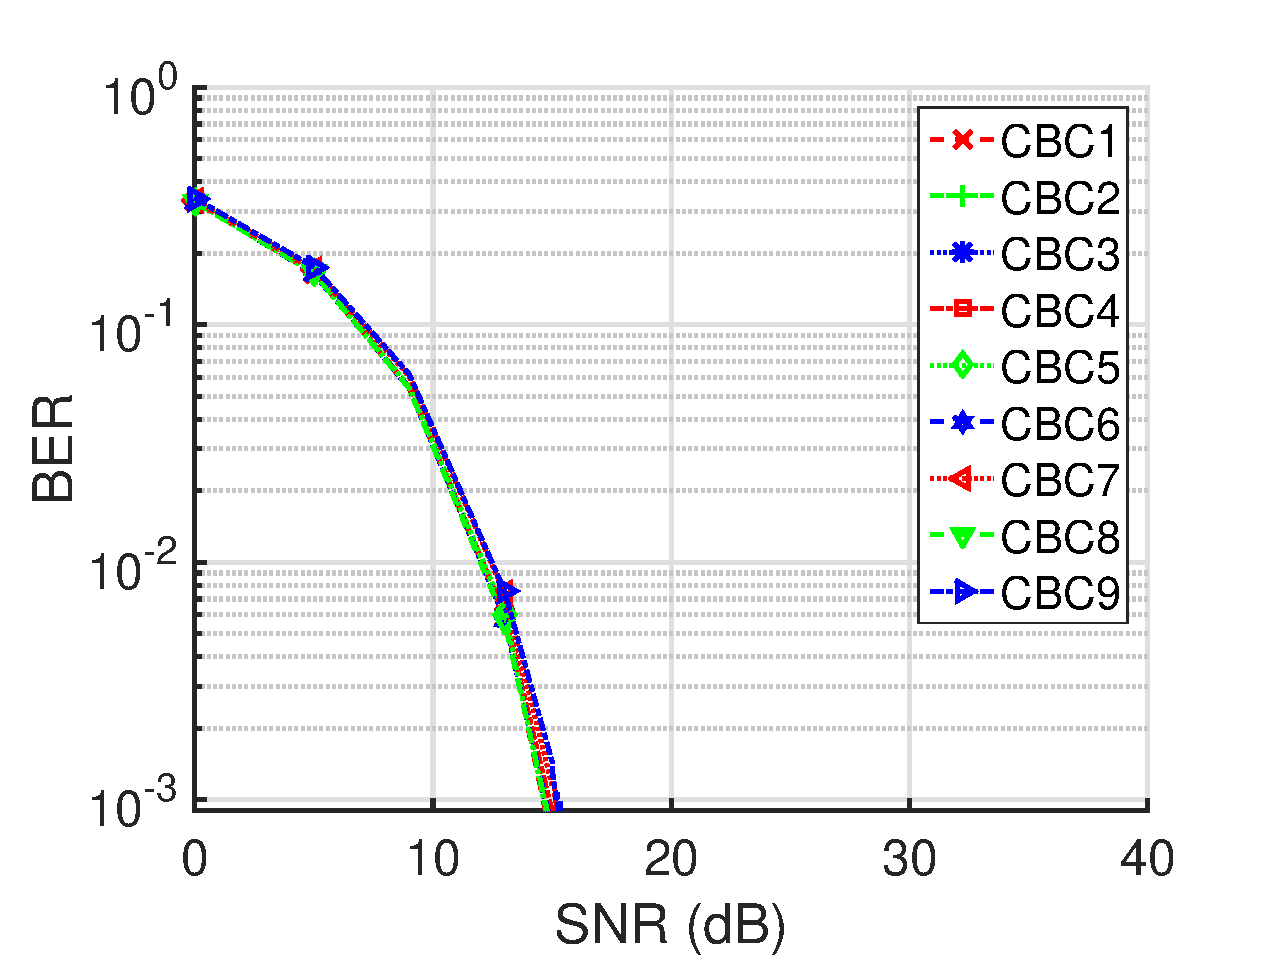
\includegraphics[trim={0.1in 0.0in 0.6in 0.3in}, clip=true, width=0.8\textwidth]{M04_4-CSK_BERvsSNR.eps}
			\caption{4-CSK}
			\label{fig4SNR}
		\end{subfigure}
		%\hfill
		\begin{subfigure}{\textwidth}
		\centering
			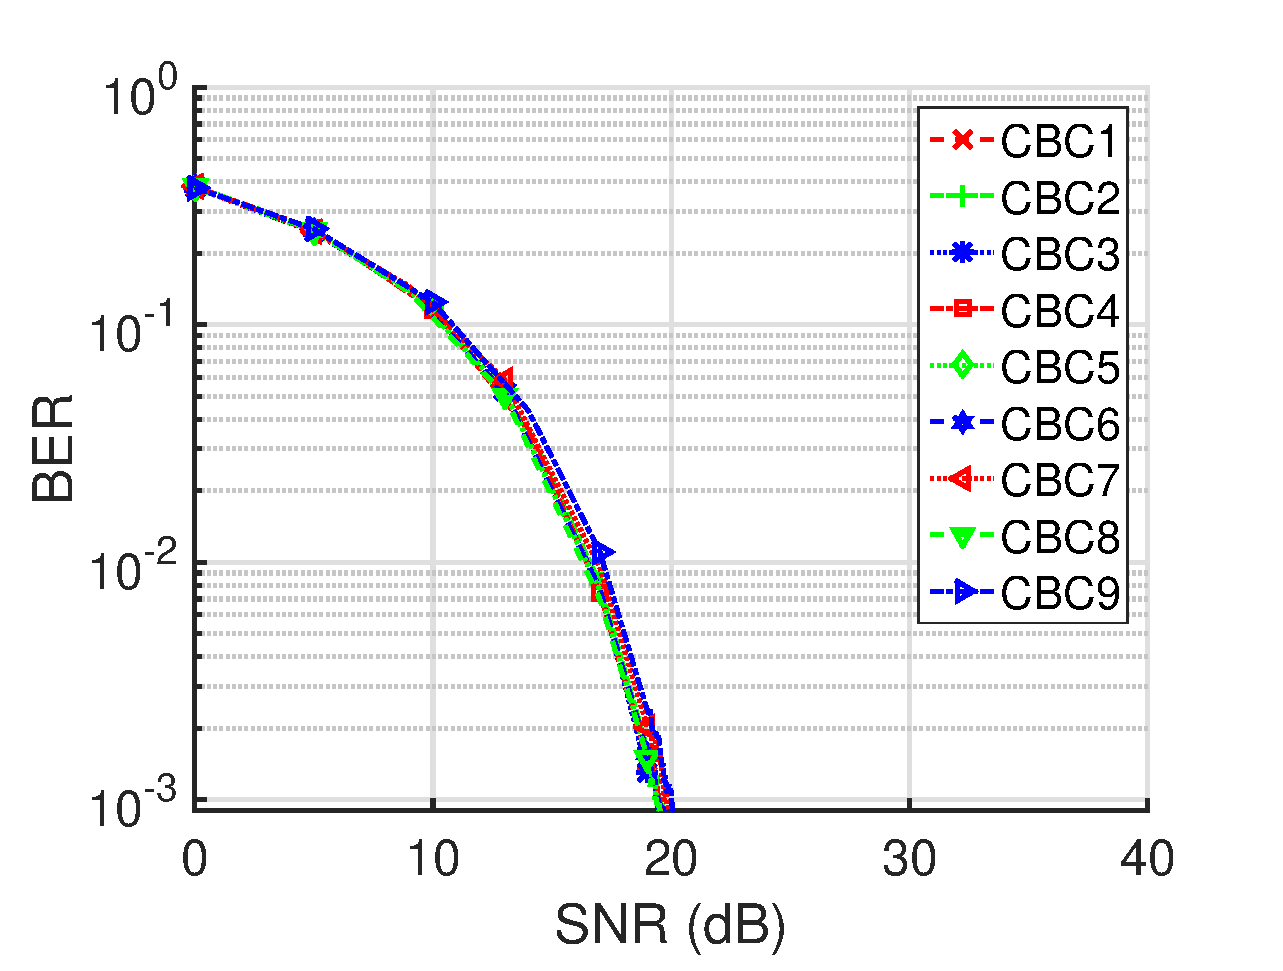
\includegraphics[trim={0.1in 0.0in 0.6in 0.3in}, clip=true, width=0.8\textwidth]{M08_8-CSK_BERvsSNR.eps}
			\caption{8-CSK}
			\label{fig8SNR}
		\end{subfigure}
		%\vfill
\end{figure}
\begin{figure}[H]
	\ContinuedFloat
		\begin{subfigure}{\textwidth}
		\centering
			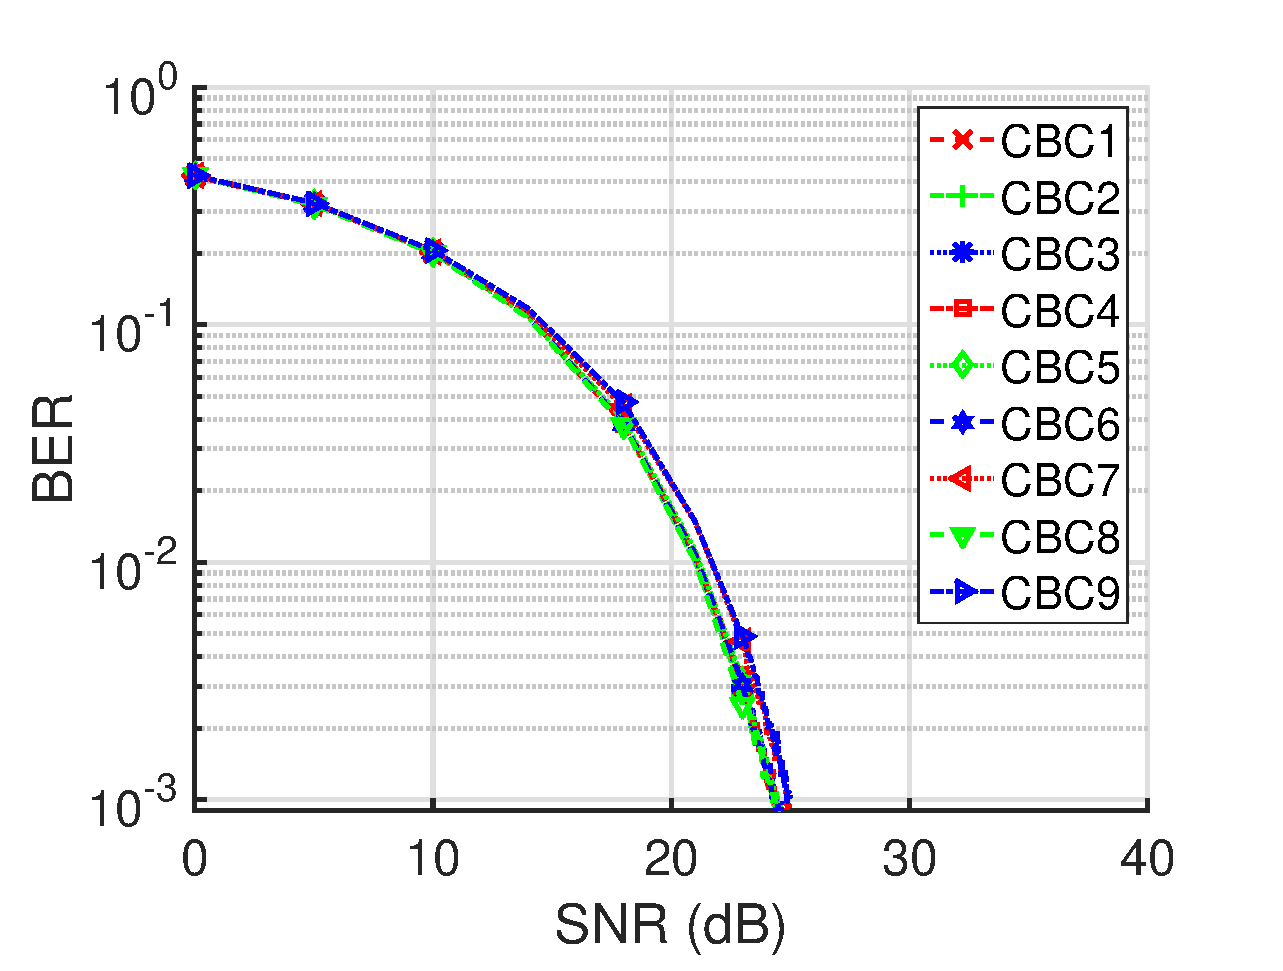
\includegraphics[trim={0.1in 0.0in 0.6in 0.3in}, clip=true, width=0.8\textwidth]{M16_16-CSK_BERvsSNR.eps}
			\caption{16-CSK}
			\label{fig16SNR}
		\end{subfigure}
	\caption{CSK linear model BER vs SNR performance for all CBCs}
	\label{figBERvsSNR}
\end{figure}
%\end{landscape}
%\clearpage% Flush page
%}

\afterpage{%
\clearpage
\begin{landscape}% Landscape page
\begin{figure}[t]
	\centering
		\begin{subfigure}{0.35\textwidth}
		\centering
			\includegraphics[trim={1.0in 0.0in 1.3in 0.1in}, clip=true, width=\textwidth]{M04_4-CSK_CBC2_ReceivedSymbols2.eps}
			\caption{4-CSK}
			\label{fig4RcvSym}
		\end{subfigure}
		%\hfill
		\begin{subfigure}{0.35\textwidth}
		\centering
			\includegraphics[trim={1.0in 0.0in 1.3in 0.1in}, clip=true, width=\textwidth]{M08_8-CSK_CBC2_ReceivedSymbols2.eps}
			\caption{8-CSK}
			\label{fig8RcvSym}
		\end{subfigure}
		%\hfill
		\begin{subfigure}{0.35\textwidth}
		\centering
			\includegraphics[trim={1.0in 0.0in 1.3in 0.1in}, clip=true, width=\textwidth]{M16_16-CSK_CBC2_ReceivedSymbols3.eps}
			\caption{16-CSK}
			\label{fig16RcvSym}
		\end{subfigure}
		\vfill
		%%%%%%%%% Y0 %%%%%%%%%
		\begin{subfigure}{0.35\textwidth}
		\centering
			\includegraphics[trim={1.0in 0.0in 1.3in 0.1in}, clip=true, width=\textwidth]{M04_4-CSK_CBC2_ReceivedSymbols2_Y0.eps}
			\caption{4-CSK}
			\label{fig4RcvSymY0}
		\end{subfigure}
		%\hfill
		\begin{subfigure}{0.35\textwidth}
		\centering
			\includegraphics[trim={1.0in 0.0in 1.3in 0.1in}, clip=true, width=\textwidth]{M08_8-CSK_CBC2_ReceivedSymbols2_Y0.eps}
			\caption{8-CSK}
			\label{fig8RcvSymY0}
		\end{subfigure}
		%\hfill
		\begin{subfigure}{0.35\textwidth}
		\centering
			\includegraphics[trim={1.0in 0.0in 1.3in 0.1in}, clip=true, width=\textwidth]{M16_16-CSK_CBC2_ReceivedSymbols3_Y0.eps}
			\caption{16-CSK}
			\label{fig16RcvSymY0}
		\end{subfigure}
	\caption[Received symbols for CSK linear model with and without clipping]{Received symbols for CBC$_{2}$ (a),(b),(c): Receiver output not clipped (d),(e),(f): Negative values of receiver output clipped at zero}
	\label{figRcvSym}
\end{figure}
%\caption{Received symbols for CBC$_{2}$.  Receiver output not clipped. (\subref{fig4RcvSym}),(\subref{fig8RcvSym}),(\subref{fig16RcvSym}): (\subref{fig4RcvSymY0}),(\subref{fig8RcvSymY0}),(\subref{fig16RcvSymY0} : Negative values of receiver output clipped at zero.}
\end{landscape}
\clearpage% Flush page
}

\figurename{ \ref{figRcvSym}} shows received symbols for CBC$_{2}$, whose constellation points are the most spread out, under the linear model. As expected, noise is spread normally along x and y dimensions forming a circular envelop around all constellation points. For $M$ = 8 and $M$ = 16, empty non-interfering regions devoid of received symbols can be seen in the figures. This indicates that these constellations could be better packed by defining additional points in the non-interfering regions. The constellations can then be further optimized to achieve better spectral efficiency. Note that in \figurename{ }\ref{figRcvSym} (\subref{fig4RcvSym}),
(\subref{fig8RcvSym}) and (\subref{fig16RcvSym}), some of the received
symbols are located outside the color gamut (triangle IJK
as outlined in \figurename{ }\ref{figConst}) formed by the sources for
i, j and k bands. This would appear to violate the relationships on the CIE-CS model between coordinates of SPDs of individual sources and that of the resultant SPD formed by mixing the fluxes in different ratios. However, at the receiver, the
received signals are influenced by noise (bipolar, zero-mean Gaussian)
resulting in bipolar received values. Received signals with negative values when mapped back to the CIE-CS, can cause received `noisy' symbols to lie outside of the gamut.

Since the transmitted radiant fluxes are always non-negative, it is possible to clip the receiver output prior to estimating the transmitted
radiant flux.  When negative receiver output is clipped at zero, estimated
symbols are illustrated in
\figurename{ }\ref{figRcvSym} (\subref{fig4RcvSymY0}),
(\subref{fig8RcvSymY0}) and (\subref{fig16RcvSymY0}). This
clipping shows that the mapping back to CIE-CS is sensical. It can also be seen that at target BER of $10^{-3}$, the clipping does not
introduce any significant change in performance when compared to that without clipping.

While this linear system model is instructive to study $M$-ary CSK modulation
and carry out a first order performance analysis, a practical CSK
system incorporating human eye's visual perception, is non-linear due to non-linearity of the CIE-CS. The ($x_{\text{p}}$, $y_{\text{p}}$) $\rightarrow  \text{P}_{n}$ block at the transmitter and its counterpart and $\hat{\text{P}}_{n}\rightarrow$ ($\hat{x}_{\text{p}}$, $\hat{y}_{\text{p}}$) at the receiver (red colored dashed
blocks in \figurename{ }\ref{figCSKBD}) introduce this non-linearity
which significantly alters the $M$-ary CSK performance for a practical
implementation. The effects of these practical constraints on a CSK
system are studied in next few sub-sections.
%%%%%%%%%%%%%%%%%%%  Non-linear Model  %%%%%%%%%%%%%%%%%%%%%
\subsection{Non-linear system model}
\label{subsec:cskNonlinear}
To understand the source of non-linearity in the CSK system, let's take a look at the CIE-CS which empirically models the human eye's visual perception of color for a stimulating SPD. Let $S_{n}(\lambda)$ be the SPDs of the transmit LEDs and P$_{n}$ be the radiant flux associated with band $n$. Thus the aggregate transmitted SPD is given by Eq.\eqref{eqWLDA}.

\begin{equation}
	W(\lambda) = \sum\limits_{n\text{ }\in\text{ \{i, j, k\}}}\text{P}_{n}S_{n}(\lambda)
	\label{eqWLDA}
\end{equation}

CIE-CS specification outlines three color matching functions - $x_{c}(\lambda)$, $y_{c}(\lambda)$ and $z_{c}(\lambda)$ as illustrated in \figurename{ }\ref{figCIEXYZ}. The tristimulus values for the three primary sources as defined in the CIE-CS are given by Eq.\eqref{eqTXYZ} and the chromaticity coordinates ($x_{\text{p}}$, $y_{\text{p}}$) of the resultant SPD $W(\lambda)$ are given by Eq.\eqref{eqWXY}. From Eqs.(\ref{eqWLDA}-\ref{eqWXY}) it can also be inferred that the relationship between P$_{n}$ and ($x_{\text{p}}$, $y_{\text{p}}$) is non-linear.

\begin{figure}[!t]
	\centering
		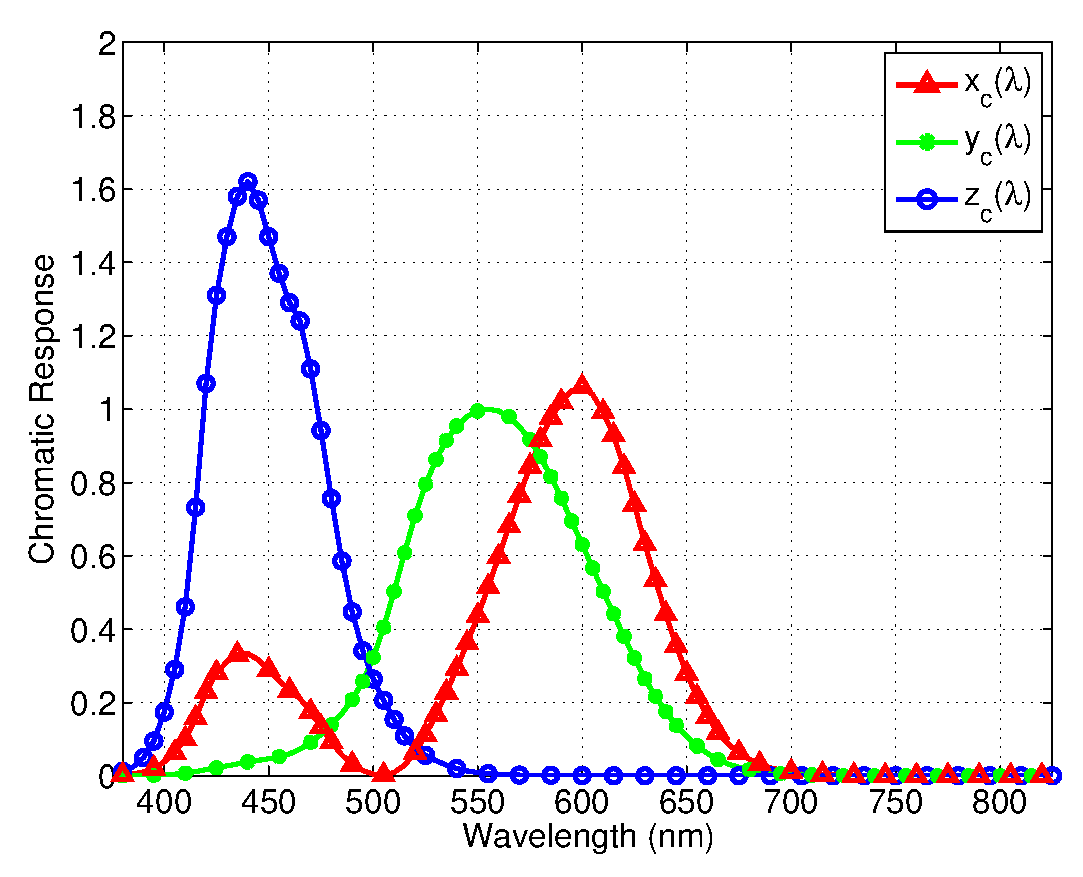
\includegraphics[trim={0.05in 0.05in 0.05in 0.05in}, clip=true, width=4.2in]{CIE1931CMF.eps}
	\caption{CIE 1931 XYZ color matching functions}
	\label{figCIEXYZ}
\end{figure}

\begin{equation}
	\begin{aligned}
		X_{W} &= \int\limits_{\lambda\text{ = 380 nm}}^{\lambda\text{ = 780 nm}}W(\lambda)x_{c}(\lambda)d\lambda\\
		Y_{W} &= \int\limits_{\lambda\text{ = 380 nm}}^{\lambda\text{ = 780 nm}}W(\lambda)y_{c}(\lambda)d\lambda\\
		Z_{W} &= \int\limits_{\lambda\text{ = 380 nm}}^{\lambda\text{ = 780 nm}}W(\lambda)z_{c}(\lambda)d\lambda
	\end{aligned}
	\label{eqTXYZ}
\end{equation}

\begin{equation}
	x_{\text{p}} = \frac{X_{W}}{X_{W}+Y_{W}+Z_{W}}; \text{  } y_{\text{p}} = \frac{Y_{W}}{X_{W}+Y_{W}+Z_{W}} % \text{  } adds space.
	\label{eqWXY}
\end{equation}

As outlined in prior sections, $M$-ary CSK modulation transmits information by varying the chromaticity coordinates of transmit SPD. In a practical implementation, a table of unique transformation ratios P$_{\text{i}}$:P$_{\text{j}}$:P$_{\text{k}}$ $\rightarrow$ $(x_{\text{p}},y_{\text{p}})$ can be pre-computed for each of the $M$ constellation points. Referring back to \figurename{ }\ref{figCSKBD}, at the transmitter the data is color coded to obtain ($x_{\text{p}}$, $y_{\text{p}}$) coordinate to transmit. Given this coordinate, corresponding flux ratios P$_{\text{i}}$:P$_{\text{j}}$:P$_{\text{k}}$ can be looked up from the pre-computed table. The target illumination requirements provide the total radiant flux to output from the transmitting sources. With the flux ratio and the total radiant flux information, individual P$_{n}$ for each band $n$ can now be computed from Eq.\eqref{eqWLDA}. This transformation now forms the ($x_{\text{p}}$, $y_{\text{p}}$) $\rightarrow  \text{P}_{n}$ block in the transmitter signaling chain. These transmitted flux are sensed by the receivers in presence of AWGN. The receivers generate an electrical output which is then used to compute an estimate of transmitted radiant fluxes $\hat{\text{P}}_{n}$. Eqs.(\ref{eqWLDA}-\ref{eqWXY}), which now constitute the $\hat{\text{P}}_{n}\rightarrow$ ($\hat{x}_{\text{p}}$, $\hat{y}_{\text{p}}$) block in the receive signal chain, can then be used to estimate the transmitted coordinate ($\hat{x}_{\text{p}}$, $\hat{y}_{\text{p}}$). Thus, the AWGN added to the received signal undergoes a non-linear transformation during $\hat{\text{P}}_{n}\rightarrow$ ($\hat{x}_{\text{p}}$, $\hat{y}_{\text{p}}$) process which skews the noise in the chromaticity plane of the CIE-CS. This causes additional performance penalties in a practical CSK system.

%\afterpage{%
%\clearpage
%\begin{landscape}% Landscape page
\begin{figure}[!t]
	\centering
		\begin{subfigure}{\textwidth}
		\centering
			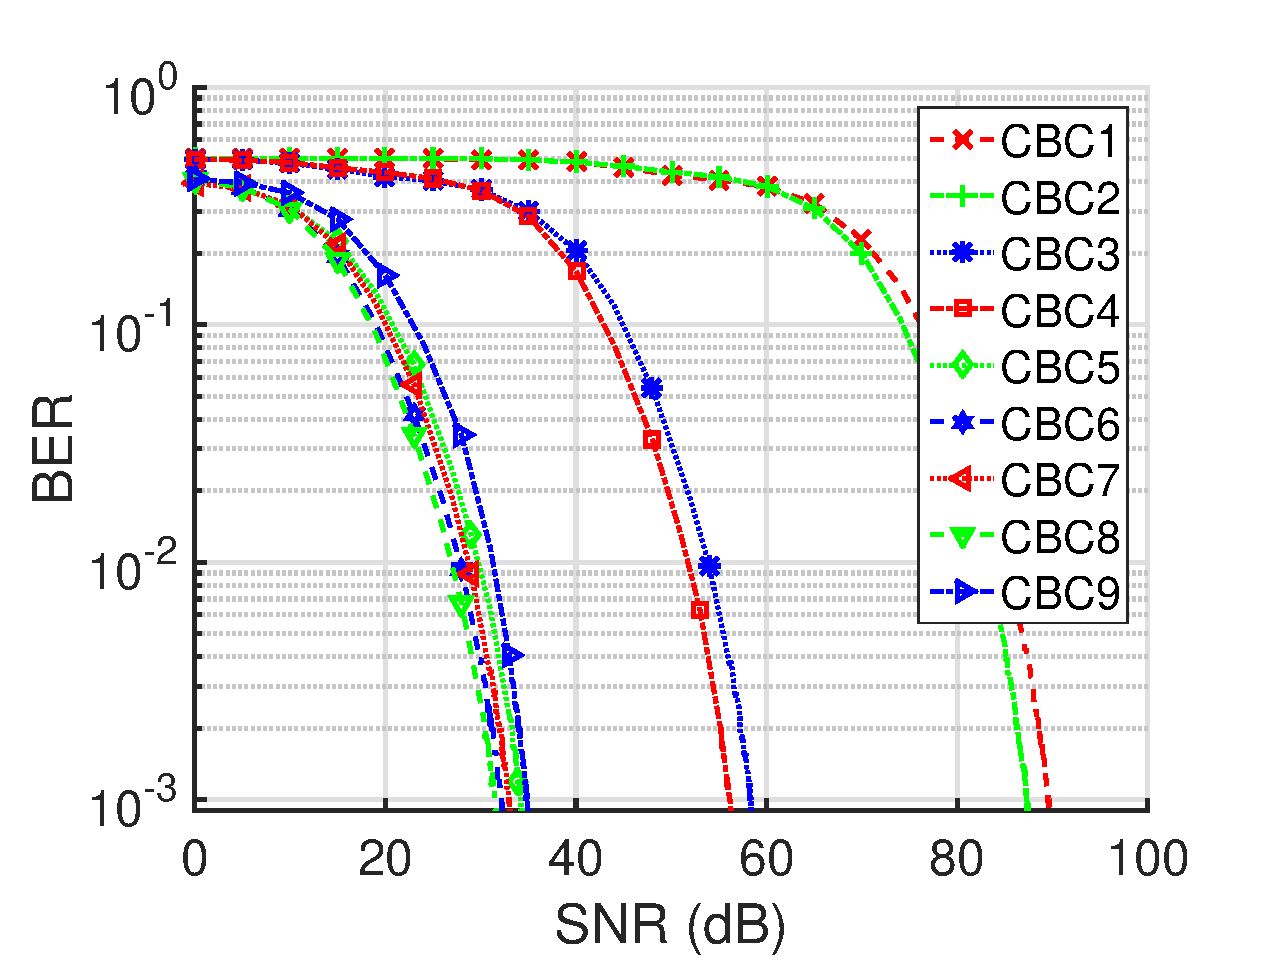
\includegraphics[trim={0.1in 0.0in 0.5in 0.3in}, clip=true, width=0.79\textwidth]{M04_4-CSK_BERvsSNR_NL.eps}
			\caption{4-CSK}
			\label{fig4SNR_NL}
		\end{subfigure}
		%\hfill
		\begin{subfigure}{\textwidth}
		\centering
			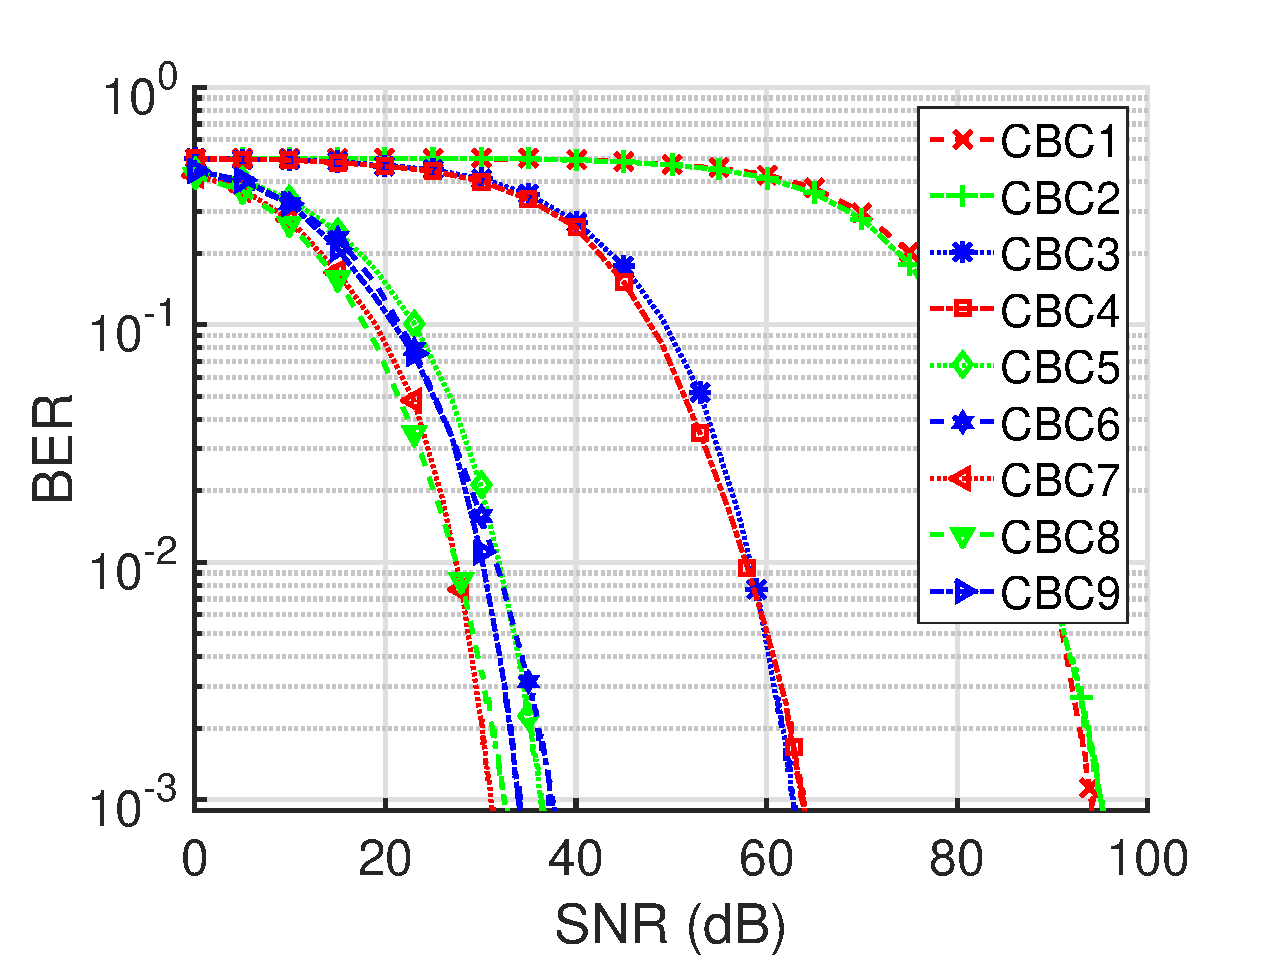
\includegraphics[trim={0.1in 0.0in 0.5in 0.3in}, clip=true, width=0.79\textwidth]{M08_8-CSK_BERvsSNR_NL.eps}
			\caption{8-CSK}
			\label{fig8SNR_NL}
		\end{subfigure}
		%\vfill
\end{figure}
%\clearpage
\begin{figure}[!t]		
	\ContinuedFloat
		\begin{subfigure}{\textwidth}
		\centering
			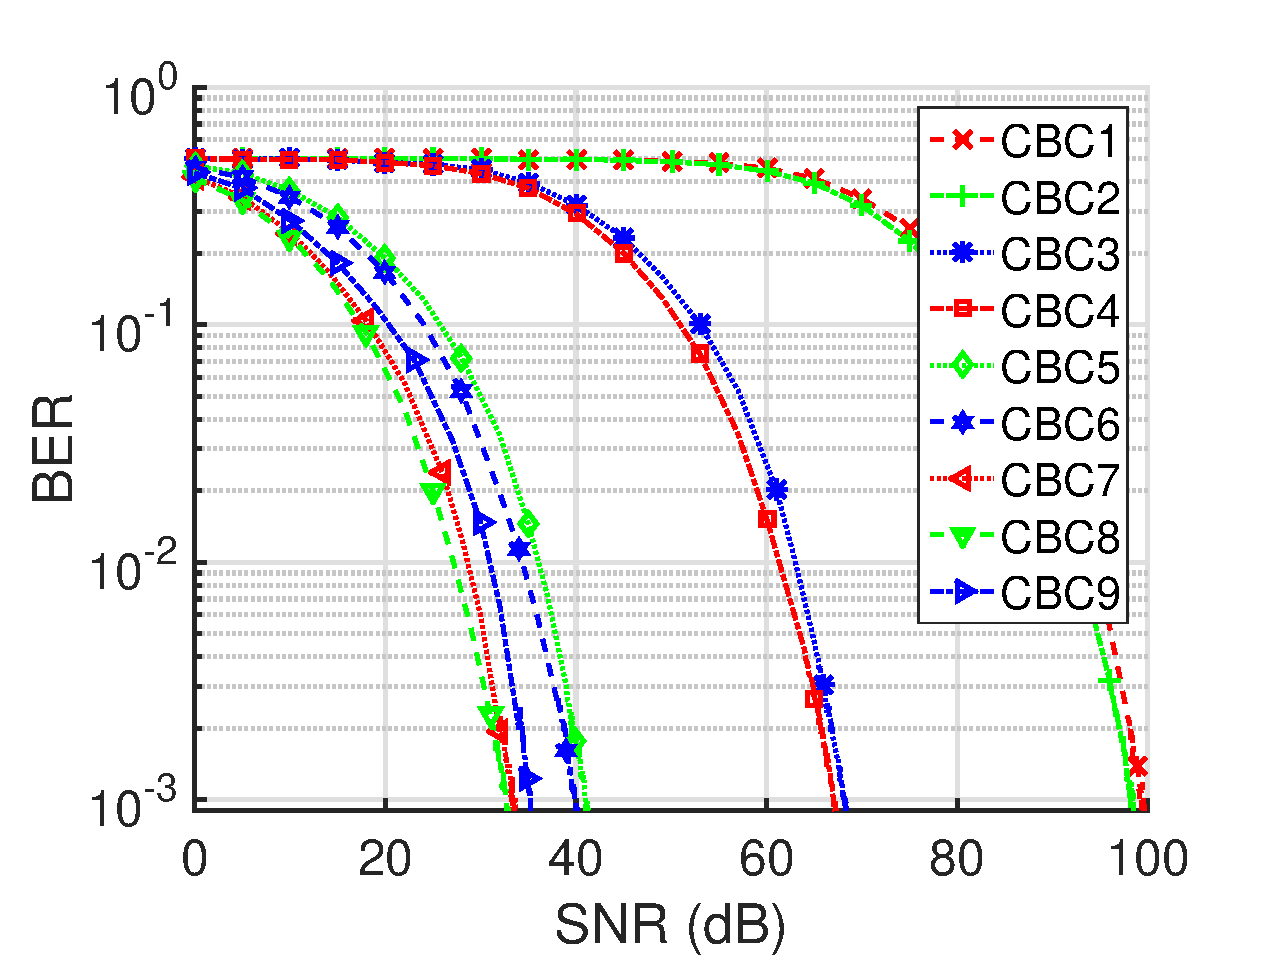
\includegraphics[trim={0.1in 0.0in 0.5in 0.3in}, clip=true, width=0.79\textwidth]{M16_16-CSK_BERvsSNR_NL.eps}
			\caption{16-CSK}
			\label{fig16SNR_NL}
		\end{subfigure}
	\caption{CSK non--linear model BER vs SNR performance for all CBCs}
	\label{figBERvsSNR_NL}
\end{figure}
%\end{landscape}
%\clearpage% Flush page
%}

\figurename{ }\ref{figBERvsSNR_NL} shows performance of all the CBCs under this non-linear model. These curves are obtained by monte-carlo simulations similar to those performed for the linear model after substituting the P$_{n}$ $\rightarrow$ ($x_{\text{p}}$, $y_{\text{p}}$) and $\hat{\text{P}}_{n}\rightarrow$ ($\hat{x}_{\text{p}}$, $\hat{y}_{\text{p}}$) blocks with the non-linear system model transformations. It can be observed that CBC$_{7}$ and CBC$_{8}$ perform relatively similar and are the best while CBC$_{1}$ performs the worst. Additionally, it is observed that CBC$_{1}$-CBC$_{4}$ perform significantly worse as compared to the rest. For CBC$_{1}$-CBC$_{4}$, the amount of radiant flux emitted by band i is 3-4 orders of magnitude greater than band j and 1-2 orders of magnitude greater than band k. Thus the $\hat{\text{P}}_{n}\rightarrow$ ($\hat{x}_{\text{p}}$, $\hat{y}_{\text{p}}$) conversion at the receiver is extremely sensitive to noise along the j and k bands as compared to that along the i band. This introduces significant errors in decoding received symbols.

\afterpage{%
%\clearpage
\begin{landscape}% Landscape page
\begin{figure}[t]
	\centering
		%%%%%%%%% CBC1 %%%%%
		\begin{subfigure}{0.35\textwidth}
		\centering
			\includegraphics[trim={1.0in 0.0in 1.3in 0.1in}, clip=true, width=\textwidth]{M04_4-CSK_CBC1_ReceivedSymbols9_NL.eps}
			\caption{CBC$_{1}$: 4-CSK}
			\label{fig4RcvSym_NL1}
		\end{subfigure}
		%%\hfill
		\begin{subfigure}{0.35\textwidth}
		\centering
			\includegraphics[trim={1.0in 0.0in 1.3in 0.1in}, clip=true, width=\textwidth]{M08_8-CSK_CBC1_ReceivedSymbols10_NL.eps}
			\caption{CBC$_{1}$: 8-CSK}
			\label{fig8RcvSym_NL1}
		\end{subfigure}
		%\hfill
		\begin{subfigure}{0.35\textwidth}
		\centering
			\includegraphics[trim={1.0in 0.0in 1.3in 0.1in}, clip=true, width=\textwidth]{M16_16-CSK_CBC1_ReceivedSymbols10_NL.eps}
			\caption{CBC$_{1}$: 16-CSK}
			\label{fig16RcvSym_NL1}
		\end{subfigure}
		%\vfill
		%%%%%%%%% CBC8 %%%%%
		\begin{subfigure}{0.35\textwidth}
		\centering
			\includegraphics[trim={1.0in 0.0in 1.3in 0.1in}, clip=true, width=\textwidth]{M04_4-CSK_CBC8_ReceivedSymbols4_NL.eps}
			\caption{CBC$_{8}$: 4-CSK}
			\label{fig4RcvSym_NL8}
		\end{subfigure}
		%\hfill
		\begin{subfigure}{0.35\textwidth}
		\centering
			\includegraphics[trim={1.0in 0.0in 1.3in 0.1in}, clip=true, width=\textwidth]{M08_8-CSK_CBC8_ReceivedSymbols4_NL.eps}
			\caption{CBC$_{8}$: 8-CSK}
			\label{fig8RcvSym_NL8}
		\end{subfigure}
		%\hfill
		\begin{subfigure}{0.35\textwidth}
		\centering
			\includegraphics[trim={1.0in 0.0in 1.3in 0.1in}, clip=true, width=\textwidth]{M16_16-CSK_CBC8_ReceivedSymbols4_NL.eps}
			\caption{CBC$_{8}$: 16-CSK}
			\label{fig16RcvSym_NL8}
		\end{subfigure}
	\caption[Received symbols for CSK non--linear model without clipping]{Received symbols for non-linear model when receiver output is not clipped}
	\label{figRcvSym_NL}
\end{figure}
%Some received symbols are located outside the color gamut. Note that noise when transformed to chromaticity plane is no longer AWGN.
\end{landscape}
%\clearpage% Flush page
}

\afterpage{%
%\clearpage
\begin{landscape}% Landscape page
\begin{figure}[t]
	\centering
	%%%%%%%%% CBC1 Y0 %%%%%
		\begin{subfigure}{0.35\textwidth}
		\centering
			\includegraphics[trim={1.0in 0.0in 1.3in 0.1in}, clip=true, width=\textwidth]{M04_4-CSK_CBC1_ReceivedSymbols9_NL_Y0.eps}
			\caption{CBC$_{1}$: 4-CSK}
			\label{fig4RcvSym_NL1_Y0}
		\end{subfigure}
		%\hfill
		\begin{subfigure}{0.35\textwidth}
		\centering
			\includegraphics[trim={1.0in 0.0in 1.3in 0.1in}, clip=true, width=\textwidth]{M08_8-CSK_CBC1_ReceivedSymbols10_NL_Y0.eps}
			\caption{CBC$_{1}$: 8-CSK}
			\label{fig8RcvSym_NL1_Y0}
		\end{subfigure}
		%\hfill
		\begin{subfigure}{0.35\textwidth}
		\centering
			\includegraphics[trim={1.0in 0.0in 1.3in 0.1in}, clip=true, width=\textwidth]{M16_16-CSK_CBC1_ReceivedSymbols10_NL_Y0.eps}
			\caption{CBC$_{1}$: 16-CSK}
			\label{fig16RcvSym_NL1_Y0}
		\end{subfigure}
		%\vfill
		%%%%%%%%% CBC8 Y0 %%%%%
		\begin{subfigure}{0.35\textwidth}
		\centering
			\includegraphics[trim={1.0in 0.0in 1.3in 0.1in}, clip=true, width=\textwidth]{M04_4-CSK_CBC8_ReceivedSymbols4_NL_Y0.eps}
			\caption{CBC$_{8}$: 4-CSK}
			\label{fig4RcvSym_NL8_Y0}
		\end{subfigure}
		%\hfill
		\begin{subfigure}{0.35\textwidth}
		\centering
			\includegraphics[trim={1.0in 0.0in 1.3in 0.1in}, clip=true, width=\textwidth]{M08_8-CSK_CBC8_ReceivedSymbols4_NL_Y0.eps}
			\caption{CBC$_{8}$: 8-CSK}
			\label{fig8RcvSym_NL8_Y0}
		\end{subfigure}
		%\hfill
		\begin{subfigure}{0.35\textwidth}
		\centering
			\includegraphics[trim={1.0in 0.0in 1.3in 0.1in}, clip=true, width=\textwidth]{M16_16-CSK_CBC8_ReceivedSymbols4_NL_Y0.eps}
			\caption{CBC$_{8}$: 16-CSK}
			\label{fig16RcvSym_NL8_Y0}
		\end{subfigure}
	\caption[Received symbols for CSK non--linear model with clipping]{Received symbols for non--linear model when negative values of receiver output are clipped at zero}
	\label{figRcvSym_NL_Y0}
\end{figure}
%All received symbols now are located inside the color gamut. Note that noise when transformed to chromaticity plane is no longer AWGN.
\end{landscape}
%\clearpage% Flush page
}

\figurename{ }\ref{figRcvSym_NL} and \figurename{ }\ref{figRcvSym_NL_Y0} show received symbols for CBC$_{1}$ and CBC$_{8}$ under the non-linear model. Noise skew about the estimated coordinates can be observed in both figures. This noise skew is more prominent for CBC$_{1}$ where the signal power distribution along all bands is imbalanced. In contrast for CBC$_{8}$, signal power is more uniformly spread across all bands. For \figurename{ }\ref{figRcvSym_NL}, the negative receiver output is not clipped at zero. As mentioned earlier, in presence of noise (zero mean and Gaussian), some receiver output values can be negative and thus such received symbols are located outside the color gamut when transformed to CIE-CS space. The effect of clipping negative receiver output at zero can be seen in \figurename{ }\ref{figRcvSym_NL_Y0} where all received symbols now are located inside the color gamut. It can be seen that performance of both receiver signal processing techniques is similar, as such no one outperforms the other. It can be seen that AWGN introduced on $\hat{\text{P}}_{n}$ gets skewed radially towards band k due to non-linearity in $\hat{\text{P}}_{n}\rightarrow$ ($\hat{x}_{\text{p}}$, $\hat{y}_{\text{p}}$) transformation and is no longer AWGN along the CIE-CS chromaticity plane. This generates an interesting outcome in that for CBC$_{8}$, about 30 dB of SNR is needed to achieve target $10^{-3}$ BER for all of $M$ = 4, 8 and 16 CSK. This happens because with increase in order $M$, the additional constellation points as defined in the standard happen to occupy non-interfering regions of the chromaticity plane thus increasing spectral efficiency without incurring any SNR penalty up to a point. The non-linearity of the CIE-CS introduces performance penalties of at least 15 dB, 10 dB and 5 dB for $M$ = 4, 8 and 16 CSK respectively over the linear system model. 

%%%%%%%%%%%%%%%%%%%%%  Illumination  %%%%%%%%%%%%%%%%%%%%%%%
\subsection{CSK system performance under illumination constraints}
\label{subsec:cskIllumination}

%%%%%%%%%%%%  Luminous Signal to Noise Ratio  %%%%%%%%%%%%%%
%\subsection{Luminous-signal-to-noise ratio}\label{ssLSNR}
In an indoor optical wireless system using lighting devices for wireless downlink access the luminaires need to simultaneously service illumination and optical wireless broadcast missions. Under this model, different colored PHY (example: different CBC$_{v}$) irradiate different amounts of radiant flux to achieve the same illumination intensity level. Thus, it is unfair to use SNR as a metric to compare performance of modulation schemes at same BER target using different colored PHY without first normalizing for illumination targets. Thus, in this section we introduce LSNR as a metric that takes into account the differences in radiant flux emitted by different PHY to achieve the same illumination intensity level. It should be noted that the LSNR metric is not specific to CSK, but instead can be used more generally to compare performance of any two optical modulation schemes that are operated at the same optical intensity levels.

Consider optical modulation scheme(s) which can be implemented with two different constellations C$_{\text{a}}$ or C$_{\text{b}}$. The fluxes emitted by the two constellations are scaled to achieve a target illumination intensity level. Let both constellations on average emit I lumens of luminous flux. Let the luminous efficacy for the two constellations be specified by $\eta_{\text{a}}$ and $\eta_{\text{b}}$ in lumens-per-watt respectively. Then the corresponding average radiant flux emitted by the two constellations is given by W$_{\text{a}}$ = I/$\eta_{\text{a}}$ and W$_{\text{b}}$  = I/$\eta_{\text{b}}$ watts respectively. Let us define a luminous ratio L$_{\text{ab}}\triangleq$ ($\eta_{\text{a}}/\eta_{\text{b}}$) $\equiv$ (W$_{\text{b}}$/W$_{\text{a}}$). Thus, for every 1 Watt of radiant flux emitted by C$_{\text{a}}$, C$_{\text{b}}$ must emit L$_{\text{ab}}$ Watt of radiant flux to achieve the same illumination intensity level. Under the model where the luminaires service illumination along with communication, it is fair to compare the performance of the two schemes at these relative radiant flux levels instead of at the absolute radiant flux levels. Thus we define the LSNR metric in Eq.\eqref{eqLSNR} as a means to compare performance of C$_{\text{b}}$ versus that of C$_{\text{a}}$ at same illumination levels. 

%\afterpage{%
%\clearpage
%\begin{landscape}% Landscape page
\begin{figure}[!t]
	\centering
		\begin{subfigure}{\textwidth}
		\centering
			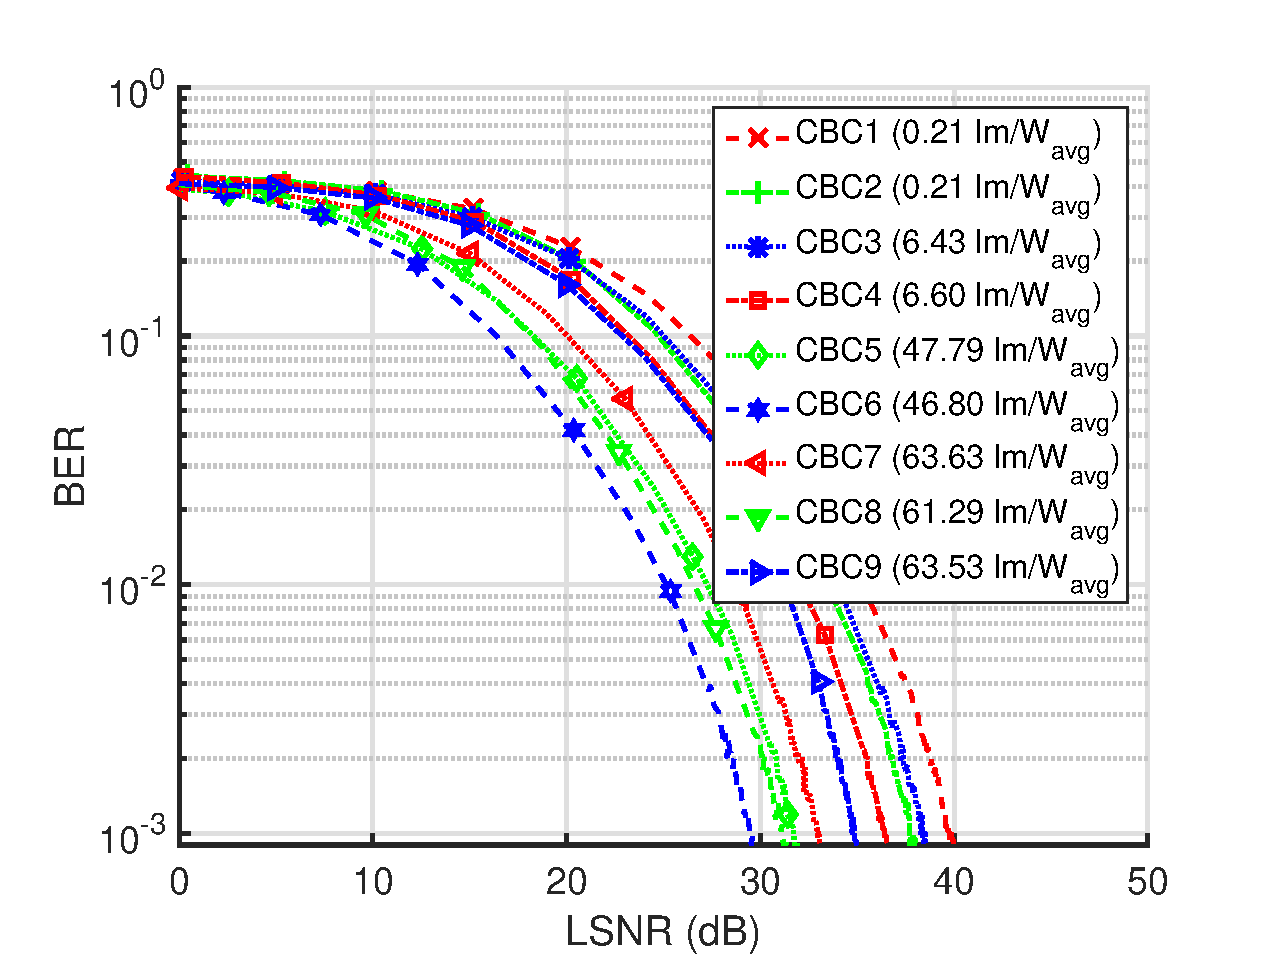
\includegraphics[trim={0.1in 0.0in 0.5in 0.1in}, clip=true, width=0.8\textwidth]{M04_4-CSK_BERvsLSNR_NL.eps}
			\caption{4-CSK}
			\label{fig4LSNR}
		\end{subfigure}
		%\hfill
		\begin{subfigure}{\textwidth}
		\centering
			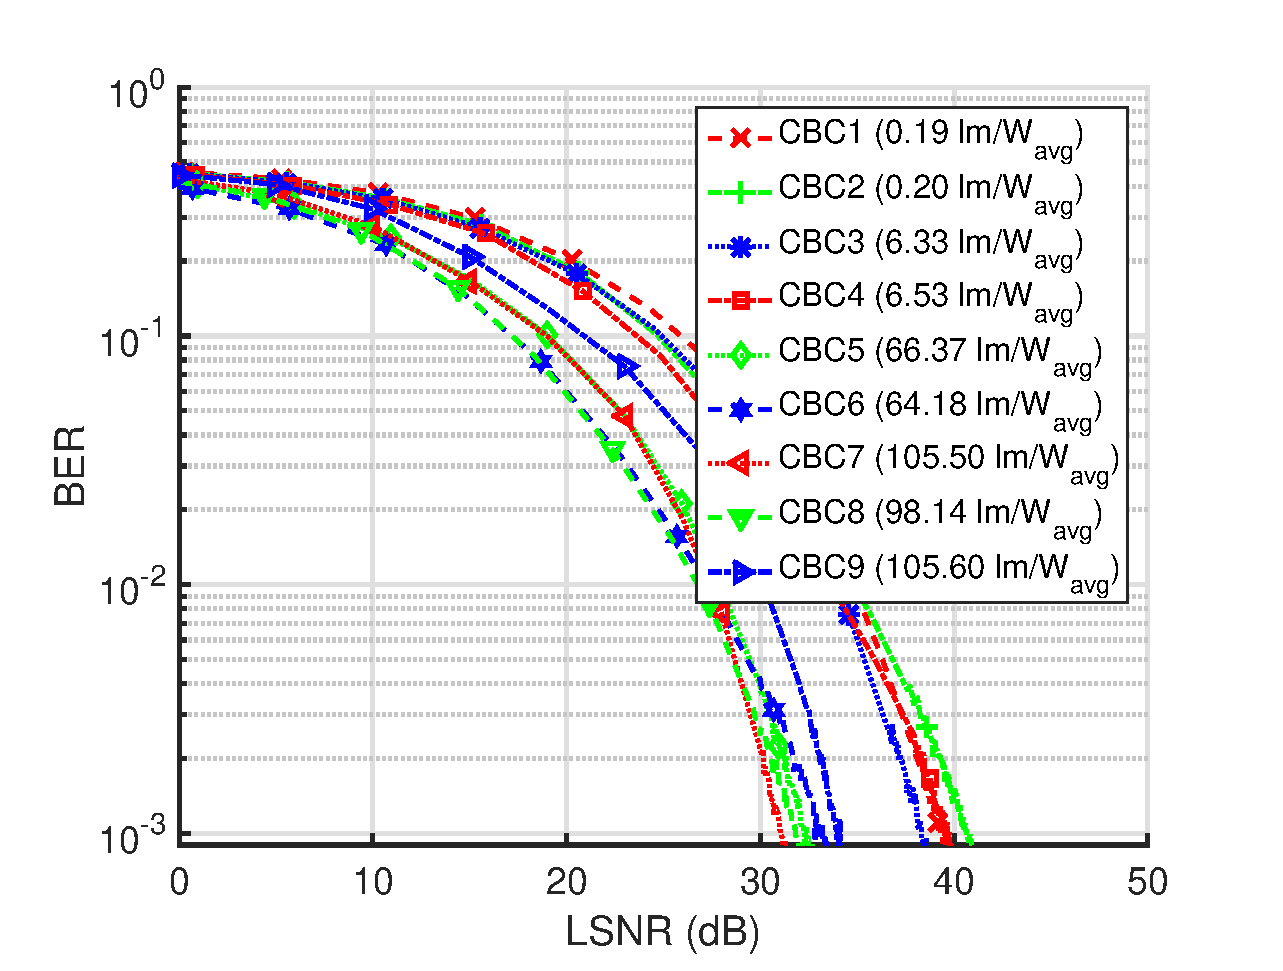
\includegraphics[trim={0.1in 0.0in 0.5in 0.1in}, clip=true, width=0.8\textwidth]{M08_8-CSK_BERvsLSNR_NL.eps}
			\caption{8-CSK}
			\label{fig8LSNR}
		\end{subfigure}
		%\vfill
	%\caption{BER vs LSNR for all CBC}
	%\label{figBERvsLSNR}
\end{figure}
\begin{figure}[!t]
	\ContinuedFloat
		\begin{subfigure}{\textwidth}
		\centering
			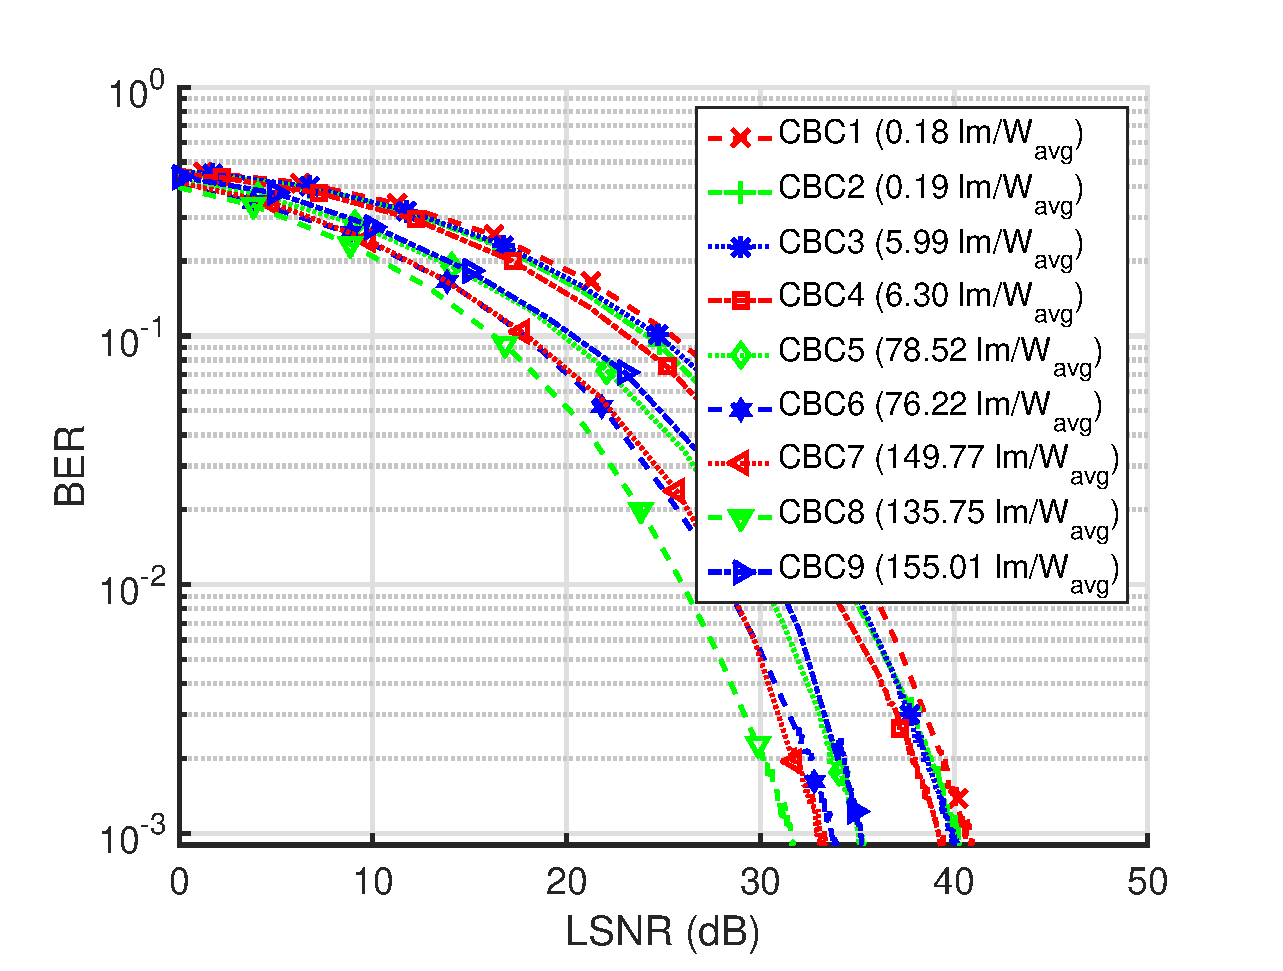
\includegraphics[trim={0.1in 0.0in 0.5in 0.1in}, clip=true, width=0.8\textwidth]{M16_16-CSK_BERvsLSNR_NL.eps}
			\caption{16-CSK}
			\label{fig16LSNR}
		\end{subfigure}
	\caption{CSK BER vs LSNR performance for all CBCs}
	\label{figBERvsLSNR}
\end{figure}
%\end{landscape}
%\clearpage% Flush page
%}


\begin{equation}
	% ^{ } is used with \vm{X} to help align subscript 'b' for both \vm{X} below.
	\text{LSNR}_{\text{ab}} \triangleq \frac{\text{L}^{2}_{\text{ab}}\text{Tr}\{\vm{H}\vm{X}^{ }_{\text{b}}\vm{X}^{*}_{\text{b}}\vm{H}^{*}\}}{\sigma^{2}_{n}} 
	\label{eqLSNR}
\end{equation}
where \vm{X}$_{\text{b}}$ is the average radiant flux emitted by C$_{\text{b}}$. Thus, after computing BER vs SNR for the scheme employing C$_{\text{a}}$, BER vs LSNR can be computed for scheme employing C$_{\text{b}}$ to compare its performance relative to that employing C$_{\text{a}}$ at the same illumination levels.

%%%%%%%%%%%%%%%%%%%%%  Illumination  %%%%%%%%%%%%%%%%%%%%%%%
%\subsection{Performance under illumination constraints}\label{ssCSKLSNR}

\figurename{ }\ref{figBERvsLSNR} shows performance of the 9 CBCs under the non-linear model when normalized for illumination constraints. The efficacies of all CBC for different $M$ are specified in the legends. These values are used to normalize the performance of $M$-ary CSK for all CBC using CBC with highest efficacy as the reference for LSNR calculation. CBC$_{7}$, CBC$_{9}$ and CBC$_{9}$ are used as reference CBCs for $M$ = 4, 8 and 16 CSK respectively. The effect of this is to shift all curves (except the reference) from \figurename{ }\ref{figBERvsSNR_NL} towards left along the LSNR-axis depending on the L$_{\text{ab}}$ values in Eq.\eqref{eqLSNR}. It can be observed that given a target illumination intensity level and for target 10$^{-3}$ BER, CBC$_{6}$ performs the best for 4-CSK, CBC$_{7}$ and CBC$_{8}$ perform similar and better than others for 8-CSK and CBC$_{8}$ performs the best for 16-CSK. For CBC$_{1}$-CBC$_{4}$, due to their low luminous efficacy, one can use a much larger radiant flux to achieve target illumination levels and thus significantly improve their communication performance. However, this is achieved at the cost of poor energy efficiency. In contrast, CBC$_{7}$ and CBC$_{9}$ have relatively high luminous efficacy. This implies that these CBCs are restricted to emit a relatively lower radiant flux (and thus low signal powers) to achieve target illumination level thus affecting their communication performance. These results also highlight the necessary tradeoff between goals of energy efficient lighting and good communication performance; thus making a case for an optimization between the two divergent goals.


% -------------------------------------
% SECTION: Metameric Modulation
% -------------------------------------
\section{Metameric modulation}
\label{sec:metameric}
\graphicspath{{_MIMOColor/figures_mm/}}

\subsection{Human eye and color perception}
\label{subsec:metamericEye}
\begin{figure}[!t]
	\centering
    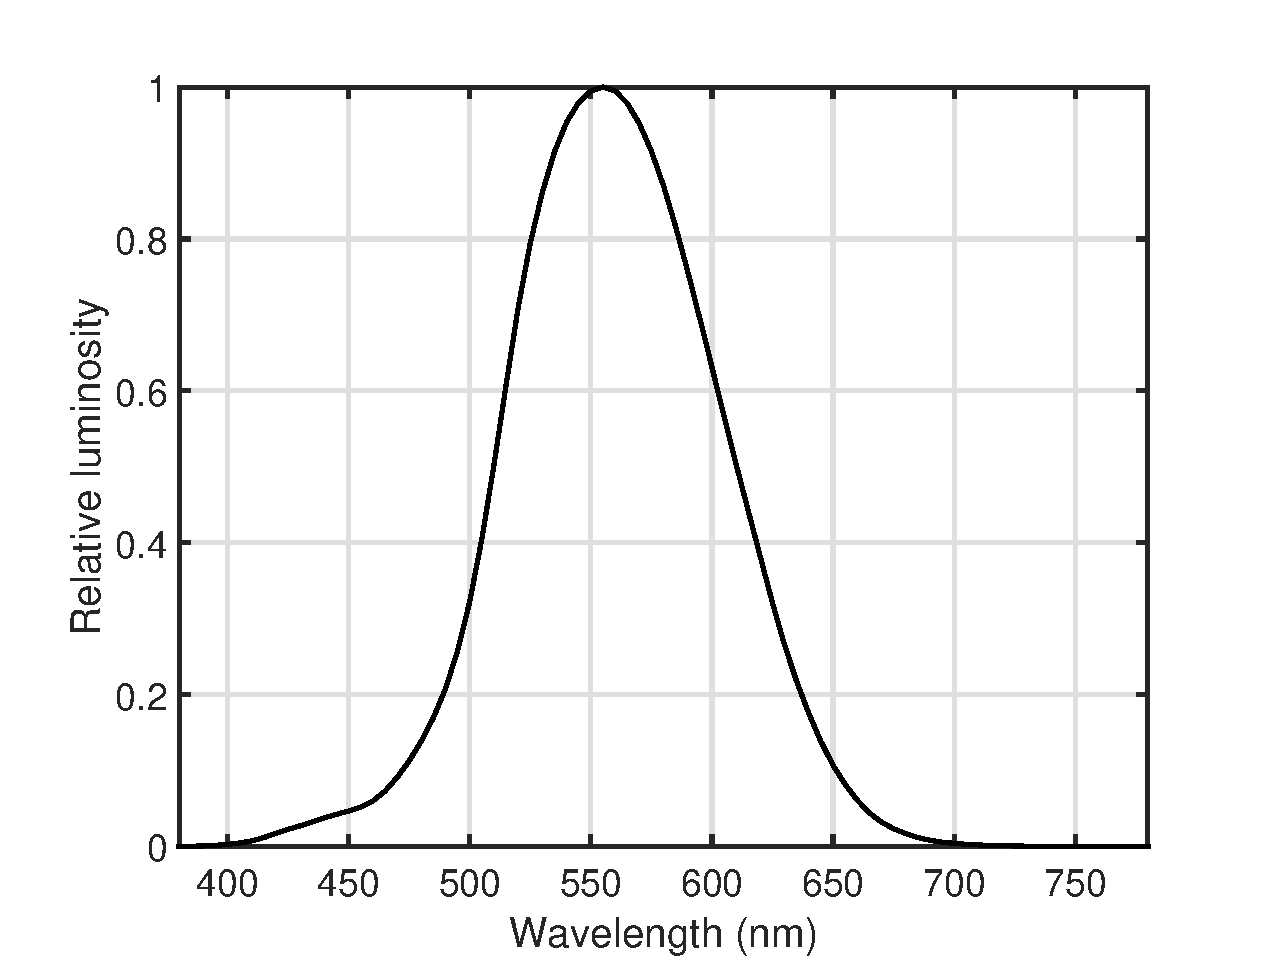
\includegraphics[trim={0.3in 0in 0.75in 0.4in}, clip=true, width=4.25in]{PhotopicResponse2.eps}
	\caption{Typical photopic relative luminous efficiency function}
	\label{figPhotopicCurve}
\end{figure}
The human eye is a sensory organ that enables humans to perceive electromagnetic radiation in a subset of the optical spectrum. \figurename{ \ref{figPhotopicCurve}} \cite{jai89a} shows the typical photopic relative luminous efficiency function of our visual system under moderate to higher levels of illumination. The retina in the eye contains sensory receptors called rods and cones. A normal human eye has three kinds of cones - short (S), medium (M) and long (L) based on the relative wavelengths that induce the peak response. Photons at different wavelengths are absorbed differently by the rods and the three sets of cones. \figurename{ \ref{figConeResp}} \cite{wan96a} shows the normalized absorbance of photons by rods and cones over a range of wavelengths. The peak responses of the cones are 420 nm, 534 nm and 564 nm while that of the rods is 498 nm. Cones are responsible for color vision. Let $S_{i}(\lambda); i\in$ \{S, M, L\}  denote their spectral responses to stimulus over a range of wavelengths. Optical stimulus with an SPD $C(\lambda)$ will induce optical sensation $\alpha_{i}$ within the cones as described in Eq. \eqref{eqAlphaCones}.
\begin{equation}
	\label{eqAlphaCones}
	\alpha_{i} = \int\limits_{0}^{\infty} C(\lambda)S_{i}(\lambda)d\lambda
\end{equation}

\begin{figure}[!t]
	\centering
%		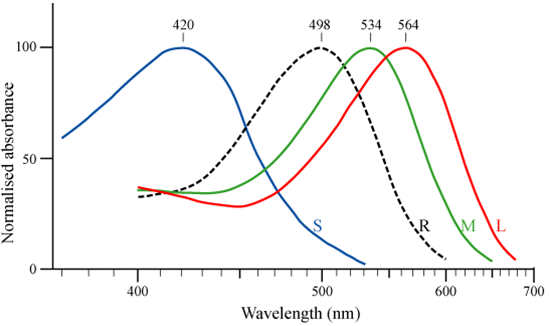
\includegraphics[width=4in]{ConeResponse.png}
    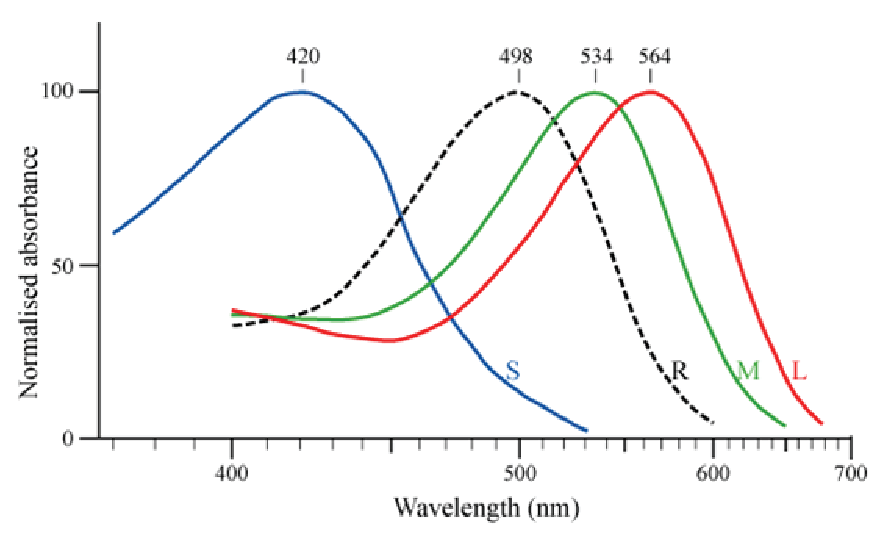
\includegraphics[width=4in]{ConeResponse.eps}
	\caption[Normalized absorbance of photons by rods and cones]{Normalized absorbance of photons by rods and cones. Ref. \cite{wan96a}}
	\label{figConeResp}
\end{figure}

Grassmann's laws \cite{gra54a} of color matching develop the theory behind the psychovisual color space spanned by cones in the human eye, henceforth called the visual color space (VCS).  This space is a subspace  of the infinite dimensional universal color space (UCS), which contains all possible SPDs. This observation leads to another interpretation of Eq. \eqref{eqAlphaCones} - the point $[{\alpha}_{\text{S}}$, ${\alpha}_{\text{M}}$, ${\alpha}_{\text{L}}]$ is a projection of a given SPD $C(\lambda)$ onto the VCS. Thus it is possible for multiple different SPDs to project onto the same point within the VCS and produce the same sensations, $[{\alpha}_{\text{S}}$, ${\alpha}_{\text{M}}$, ${\alpha}_{\text{L}}]$, in the human eye. These SPDs are sensed as the same color by the human eye and are called metamerically equivalent. Light from three independent primary light sources can be mixed in varying amounts to generate arbitrary colors. Let's call this resulting color space the primary color space (PCS). The projection of the PCS onto the VCS is called the color gamut of the primaries.

Section \ref{subsec:cskNonlinear} provides a mathematical model that incorporates visual perception and maps SPDs to a point on the chromaticity plane. Since metamerically equivalent SPDs generate the same sensation from human eye, they are mapped to the same chromaticity point on the CIE-CS. The color gamut on the CIE-CS is a polygon with chromaticity coordinate of the primary light sources as its vertices.

\subsection{MM system outline}
\label{subsec:metamericMM}
Metameric modulation (MM) is implemented by using multiple sets of primary light sources capable of providing user requested illumination color.
\begin{figure}[!t]
	\centering
    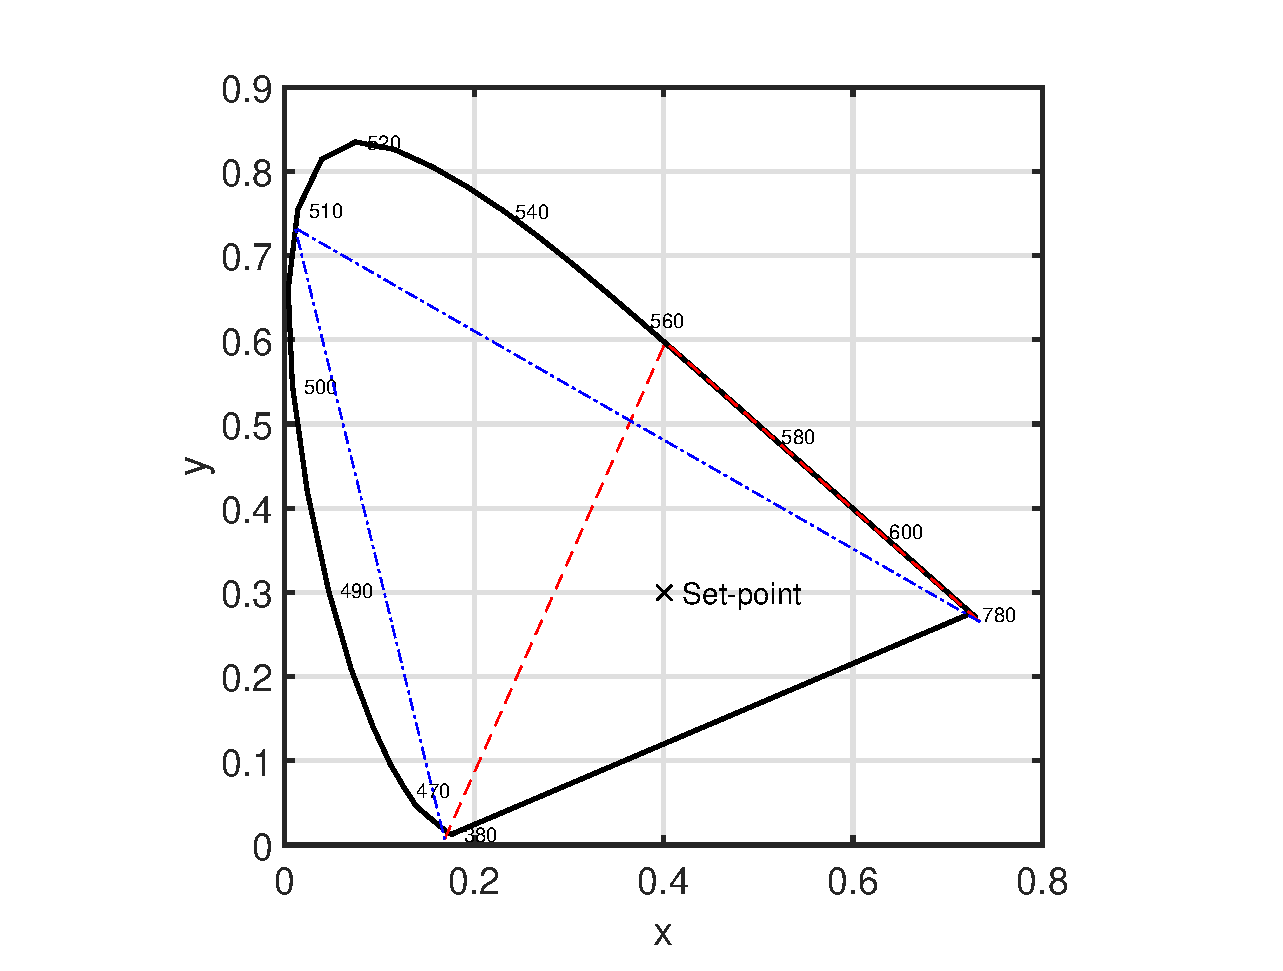
\includegraphics[width=4in]{CIE_XYZ_MM2.eps}
	\caption{Example gamuts for MM with $D=4$, $K=3$ and $M=2$}
	\label{figCIEXYZMM}
\end{figure}
If we have $D$ sources and each primary set is rendered with $K$ primary elements, there are $\binom{D}{K}$ possible primary sets. As the number of primary sets increases, the intersection of their color gamuts quickly approaches an empty set. However only $M$ of the possible primary sets are selected so that the intersection of their color gamuts contain all of the desired lighting states. \figurename{ \ref{figCIEXYZMM}} shows an example for $D=4$, $K=3$ and $M=2$. The two sets of primaries, [Blue, Cyan, Red] and [Blue, Green, Red] have a significant overlap in their color gamuts. In this case they are capable of generating a set point with two different metameric SPDs. 

%\begin{figure}[!t]
	%\centering
%%		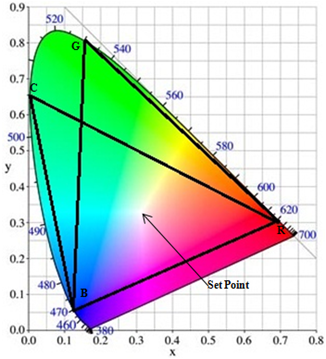
\includegraphics[width=2.5in]{CIE_XYZ_MM.png}
    %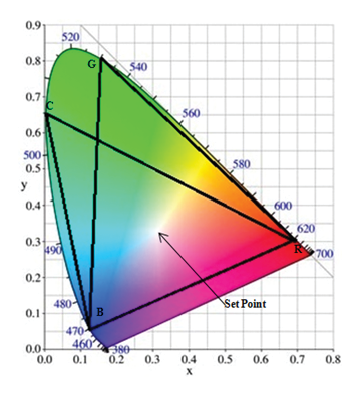
\includegraphics[width=2.5in]{CIE_XYZ_MM.eps}
	%\caption{Example gamuts for MM with $D=4$, $K=3$ and $M=2$}
	%\label{figCIEXYZMM}
%\end{figure}

MM requires detection and discrimination of multiple wavelengths at the receiver. The necessary photodiodes must be designed such that when different primaries are activated to generate a desired ambient color, the receiver can detect which primary set is active while the lighting state appears the same to the human eye. The following derivation details how this can be achieved. 

Consider $K=3$ independent light sources that form one set of primaries. Let each $L_{k}(\lambda)$ be the normalized emission spectra of the $k^{th}$ source such that Eq. \eqref{eqNormEmm} holds.
\begin{equation}
	\label{eqNormEmm}
	\int\limits_{0}^{\infty} L_{k}(\lambda)d\lambda = 1
\end{equation}

Let $\alpha_{i}^{k}$ (\ref{eqAlphaPrimaries}) be the spectral response induced by the $k^{th}$ primary on the $i^{th}$ class of cones.
\begin{equation}
	\label{eqAlphaPrimaries}
	\alpha_{i}^{k} = \int\limits_{0}^{\infty} L_{k}(\lambda)S_{i}(\lambda)d\lambda
\end{equation}

Let $C(\lambda)$ be the SPD of the ambient color that we wish to maintain. Let each $\beta_{k}$ be the amount of the corresponding $L_{k}(\lambda)$ needed to metamerically match $C(\lambda)$. Let $\alpha_{i}^{'}$ (\ref{eqAlphaPrime}) be the aggregate response evoked by the primaries on the $i^{th}$ class of cones. Grassmann's laws of color matching uphold the linearity property of color addition over a wide range of luminances. Our typical ambient illuminance levels lie well within this range of luminances.
\begin{equation}
	\label{eqAlphaPrime}
	\alpha_{i}^{'} = \sum\limits_{k=1}^{K} \beta_{k}\alpha_{i}^{k}
\end{equation}

The primaries must collectively evoke the same spectral responses in the human eye to match the color that is sensed due to $C(\lambda)$. Equating $\alpha_{i}$ in (\ref{eqAlphaCones}) with $\alpha_{i}^{'}$ in (\ref{eqAlphaPrime}) $\forall i$ leads to the color matching equation (\ref{eqColorMatch}). Solving for $\beta_{k}$ gives the relative amount of each primary that is needed to achieve a metamerical match with $C(\lambda)$.
\begin{equation}
	\label{eqColorMatch}
	\sum\limits_{k=1}^{K} \beta_{k}\int\limits_{0}^{\infty} L_{k}(\lambda)S_{i}(\lambda)d\lambda = \int\limits_{0}^{\infty} C(\lambda)S_{i}(\lambda)d\lambda
\end{equation}

Let $W(\lambda)$ be the SPD of the reference white against which the LEDs are calibrated. Let $w_{k}$ be the amount of $L_{k}(\lambda)$ needed to metamerically match $W(\lambda)$. Each tristimulus value, $t_{k}$, of each primary is defined in (\ref{eqTristimulus}). Varying $t_{k}$ for each primary changes the relative amount of the light output from each source that is mixed and thus changes color.
\begin{equation}
	\label{eqTristimulus}
	t_{k} = \beta_{k}/ w_{k}
\end{equation}

Let the individual emission spectra of the $k^{th}$ source from the $m^{th}$ set of primaries be  $L_{k}^{m}(\lambda)$. Now, let us assume we have $P$ receivers selected as mentioned above. Let the effective receiver spectral responses be $S_{p}^{'}(\lambda)$. This includes filter transmittance, concentrator gain and responsivity of the sensor and can be computed similar to Eq. \eqref{eqReff} for a normalized white spectrum. When light from all sources of the $m^{th}$ set of primaries is incident on the $p^{th}$ photodiode, its current output, $I_{p}^{m}$, is given by (\ref{eqPDCurrent}). 
\begin{equation}
	\label{eqPDCurrent}
	I_{p}^{m} = \sum\limits_{k=1}^{K} \beta_{k}\int\limits_{0}^{\infty} L_{k}^{m}(\lambda)S_{p}^{'}(\lambda)d\lambda
\end{equation}

For a given color, the response matrix $R_{g}$ is given by (\ref{eqRespMatrix}). It is possible to design a system where every column of matrix $R_{g}$ would be distinct. One way of achieving this is by using optical filters with their peak transmittance aligned with peak primary source emissions. Optimal estimation of active primary set can be made by comparing output of the photodiodes with the columns of $R_{g}$.
\begin{equation}
	\label{eqRespMatrix}
R_{g} = \left( \begin{array}{ccc}
I_{1}^{1}&\cdots&I_{1}^{M}\\
\vdots&\ddots&\vdots\\
I_{P}^{1}&\cdots&I_{P}^{M}
\end{array} \right)
\end{equation}

\begin{figure}[!b]
	\centering
%		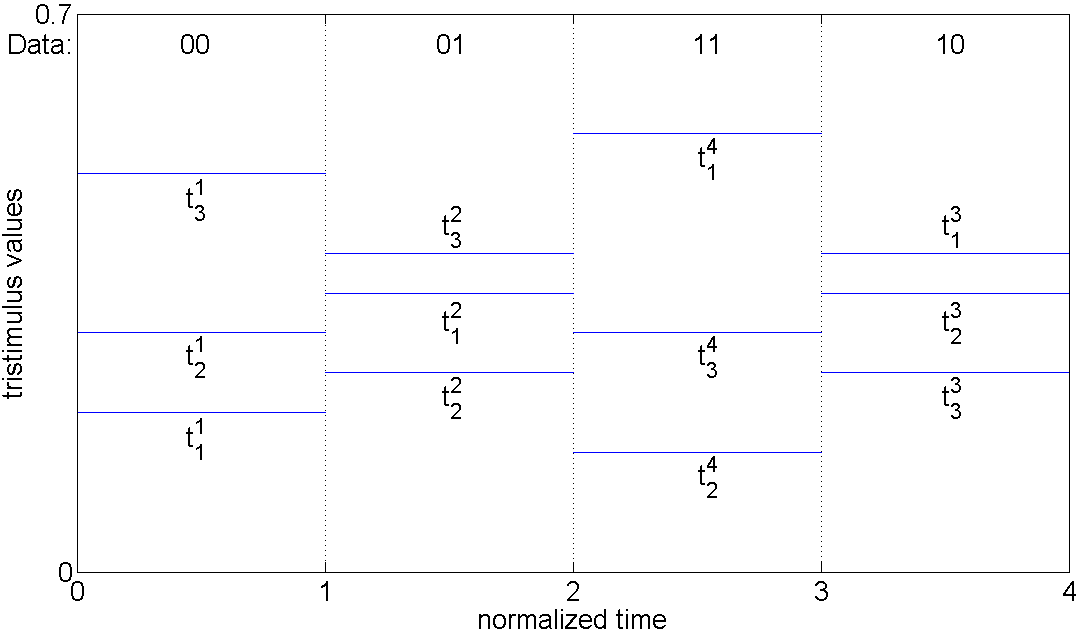
\includegraphics[width=5in]{MM_time.png}
    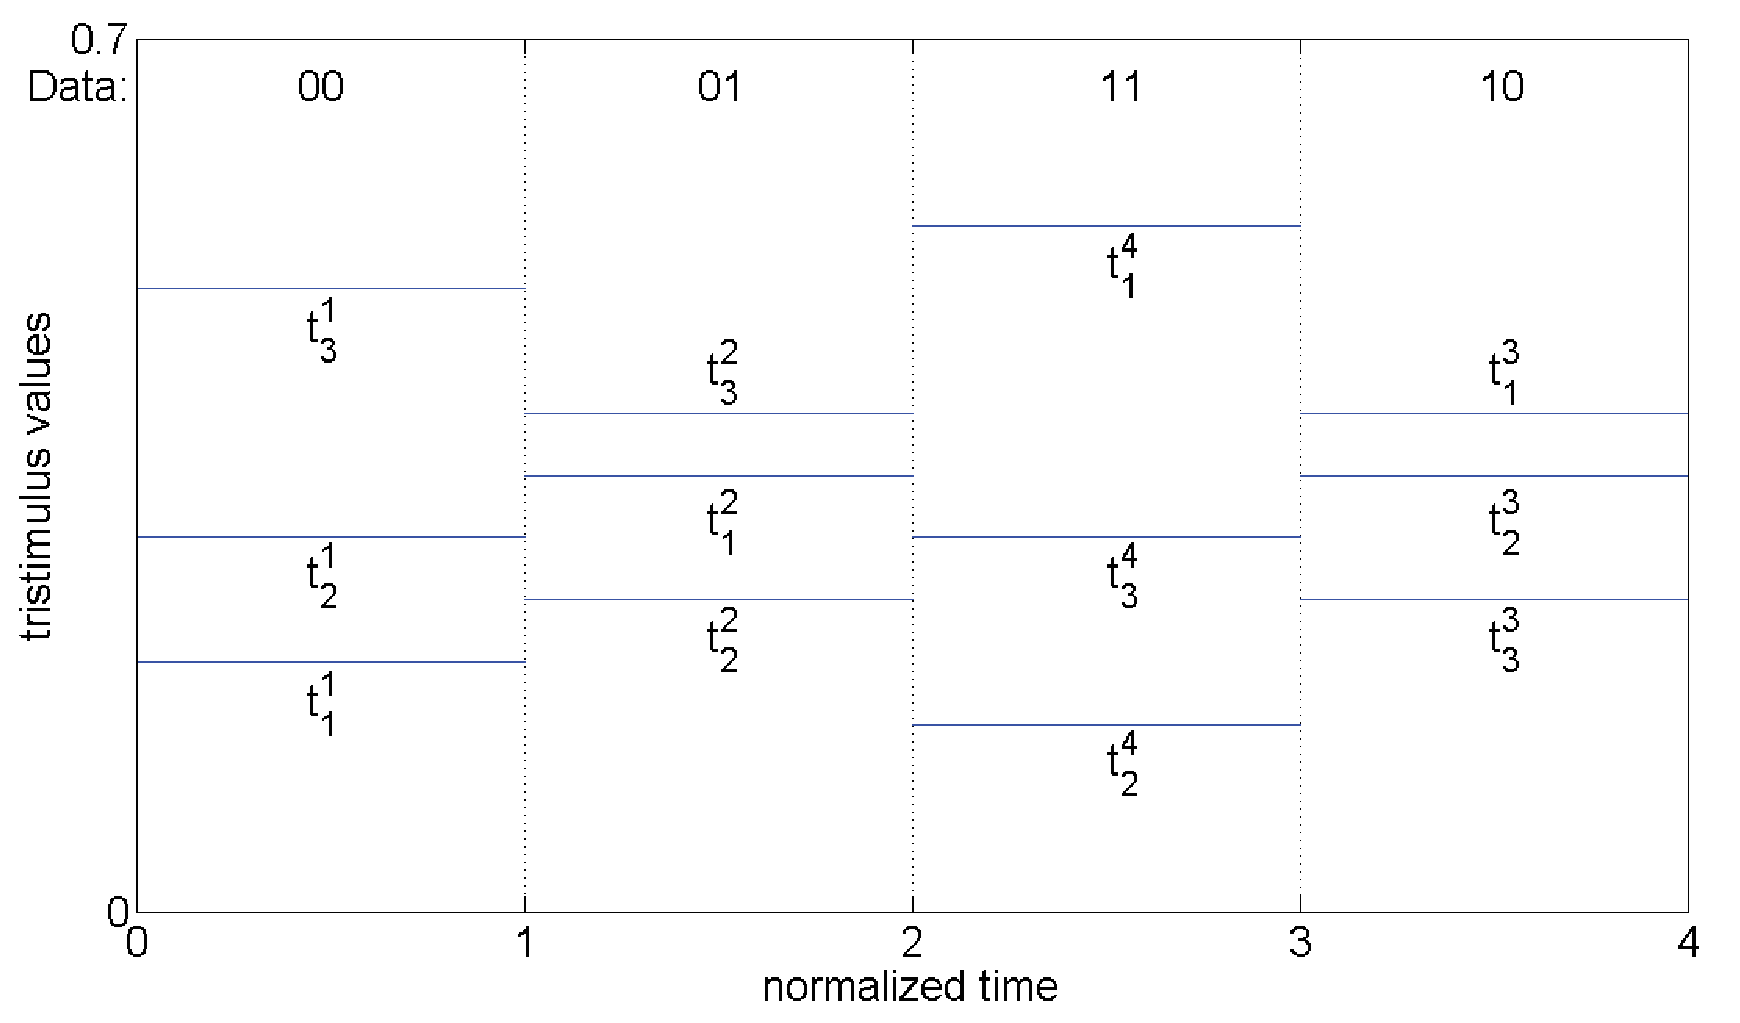
\includegraphics[width=5in]{MM_time.eps}
	\caption[MM example timing diagram]{MM example timing diagram. Illustrates different metamerically equivalent SPDs being transmitted in different time slots.}
	\label{figMMex}
\end{figure}

\begin{table}[!t]
	\centering
		\begin{tabular}{|c|c|}
		\hline
		{Primary Set Index} & {Symbol}\\
		\hline
		1 & 00\\
		2 & 01\\
		3 & 10\\
		4 & 11\\
		\hline
		\end{tabular}
	\caption{MM symbol mapping}
	\label{tblMMSymbol}
\end{table}

The desired ambient lighting state can be specified by a point on the chromaticity plane of the standard CIE-CS. Table \ref{tblMMSymbol} shows example symbol map for $M=4$. CIE-CS color space transforms can then be applied to specify the desired color within the $M$ individual primary sets. Let $t_{k}^{m}$ be the tristimulus value of the $k^{th}$ primary of the $m^{th}$ primary set. These primary sets can now generate distinct but metamerically equivalent SPDs. Switching between the different primary sets transmits symbols.

\figurename{ \ref{figMMex}} illustrates MM using these primary sets to transmit a part of an encoded information stream $(00011110_{2})$. This is accomplished by switching primaries in the order 1-2-4-3. This order can then be detected by analyzing the received signal vector and data can be decoded. The embedded MM modulation is invisible to humans due to metamerism.
%%%%%%%%%%%%%%%%%%%%%%%%%%%%%%%%%%%%%%%%%%%%%%%%%%%%%%%%%%%%%%%%%%%%%%
%%%%%%%%%%%%%%%%%%%%%%%%%%%%%%%%%%%%%%%%%%%%%%%%%%%%%%%%%%%%%%%%%%%%%%
%%%%%%%%%%%%%%%%%%%%%%%%%%%%%%%%%%%%%%%%%%%%%%%%%%%%%%%%%%%%%%%%%%%%%%
\subsection{MM system performance}
\label{subsec:metamericPerformance}

\begin{figure}[t]
	\centering
    
\includegraphics[trim={0in 0in 0in 0in}, clip=true, width=\textwidth]{MMBlockDiagram.png}
	\caption{MM block diagram using IEEE 802.15.7 CBCs}
	\label{figMMBD}
\end{figure}

\afterpage{%
%\clearpage
\begin{figure}[H]
	\centering
		\begin{subfigure}{\textwidth}
		\centering
			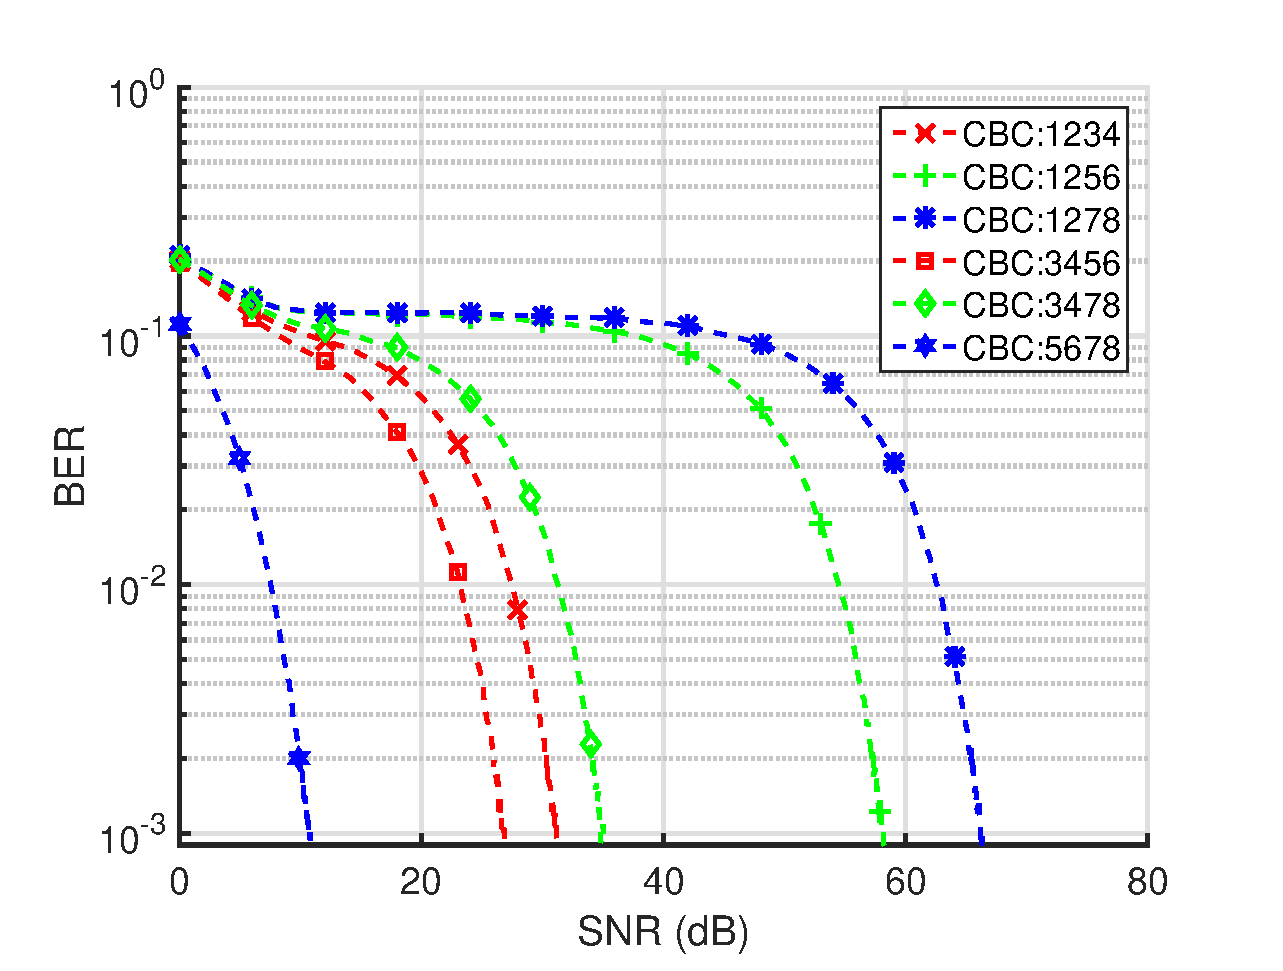
\includegraphics[trim={0.1in 0.0in 0.5in 0.1in}, clip=true, width=0.79\textwidth]{M4_N5_4-MM_BERvsSNR.eps}
			\caption{4-MM, $D$=5}
			\label{fig4MM5}
		\end{subfigure}
		%\hfill
		\begin{subfigure}{\textwidth}
		\centering
			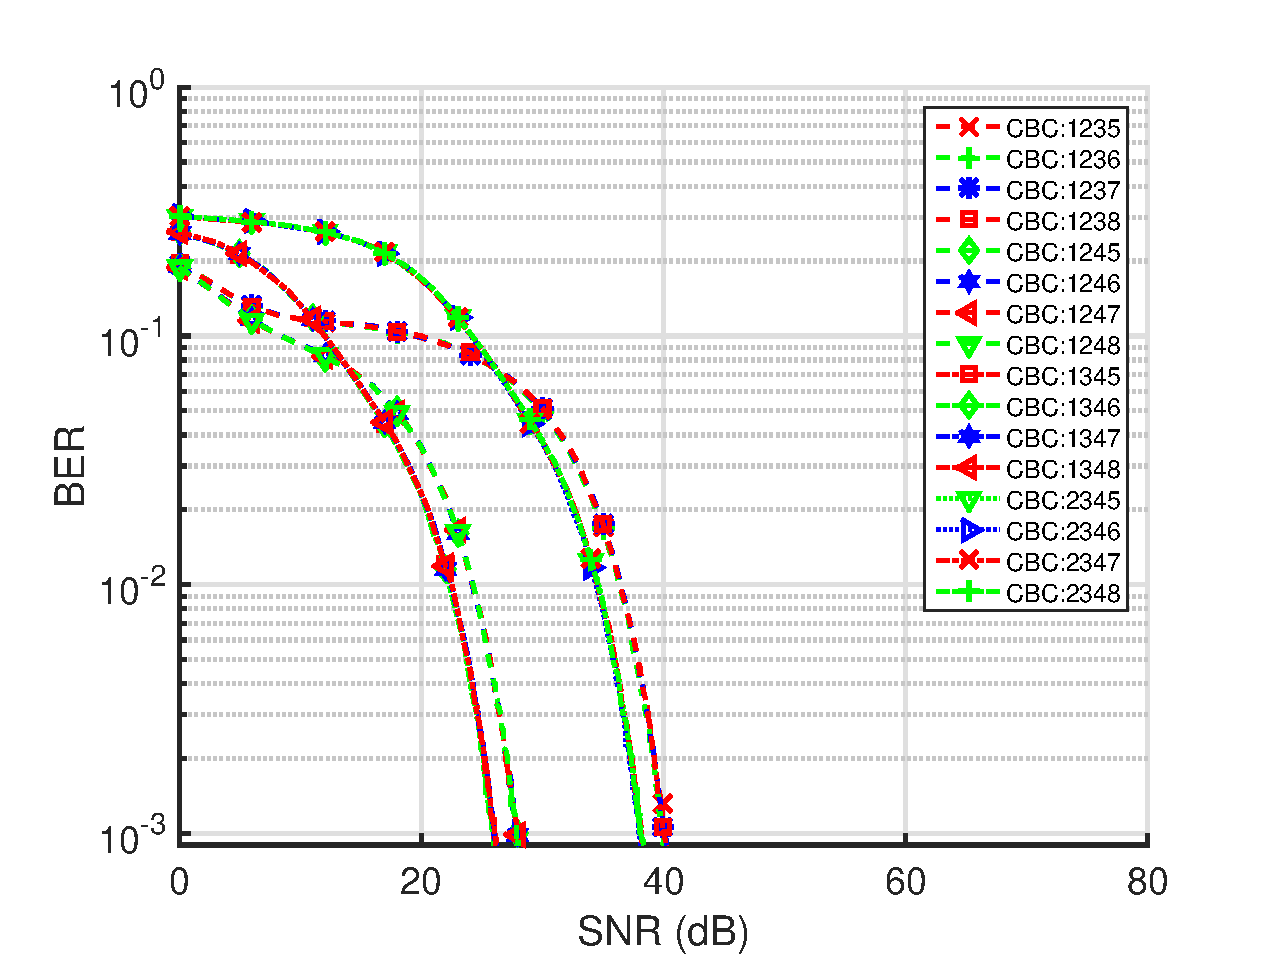
\includegraphics[trim={0.1in 0.0in 0.5in 0.1in}, clip=true, width=0.79\textwidth]{M4_N6_4-MM_BERvsSNR.eps}
			\caption{4-MM, $D$=6}
			\label{fig4MM6}
		\end{subfigure}
		%\vfill
		%\caption{BER vs SNR for different combinations of CBC}
	%\label{figMM_BERvsSNR}
\end{figure}
\begin{figure}[H]
		\ContinuedFloat
		\begin{subfigure}{\textwidth}
		\centering
			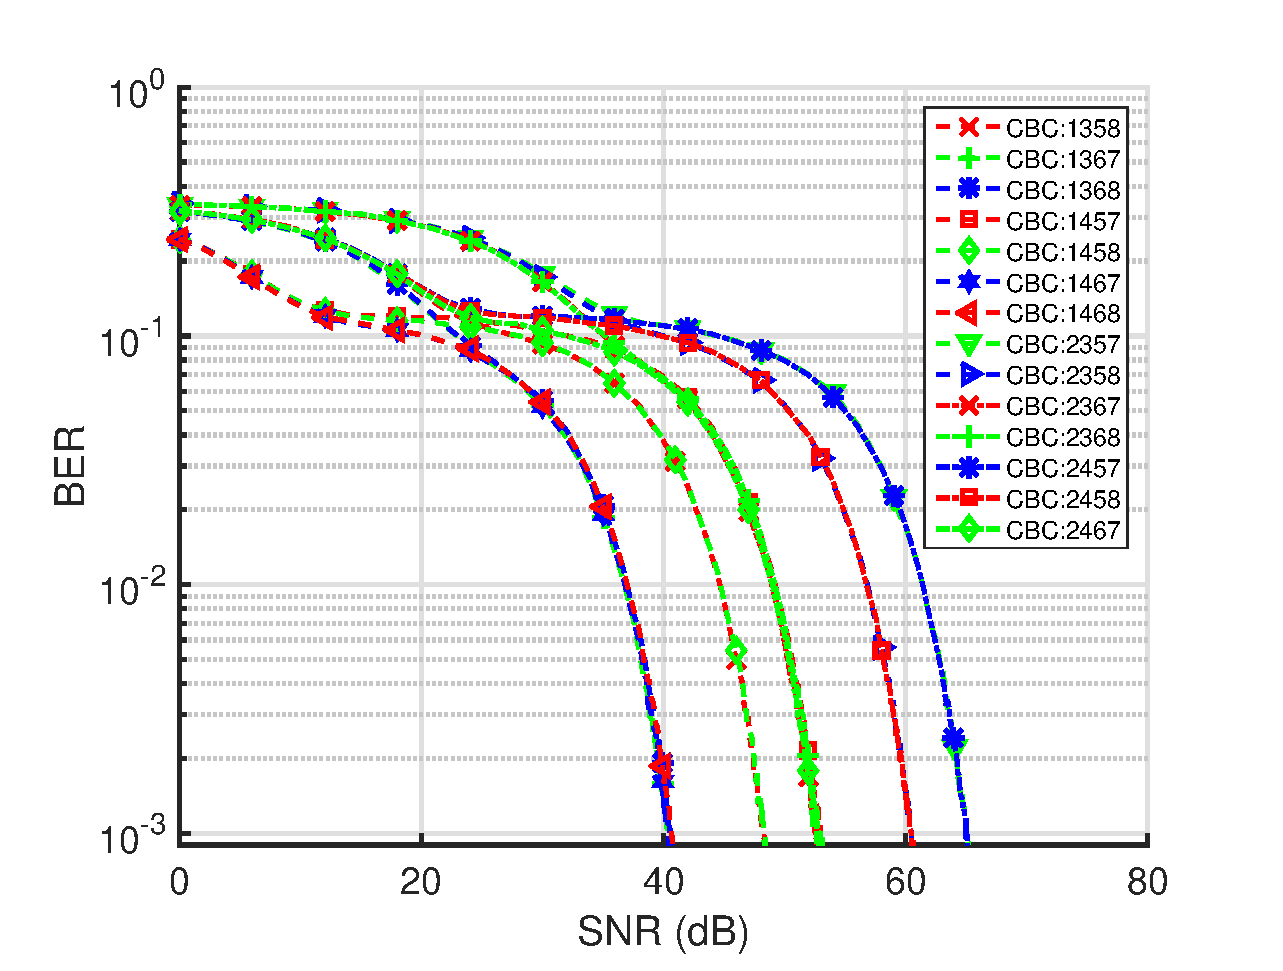
\includegraphics[trim={0.1in 0.0in 0.5in 0.1in}, clip=true, width=0.79\textwidth]{M4_N7_4-MM_BERvsSNR.eps}
			\caption{4-MM, $D$=7}
			\label{fig4MM7}
		\end{subfigure}
		%\hfill
		\begin{subfigure}{\textwidth}
		\centering
			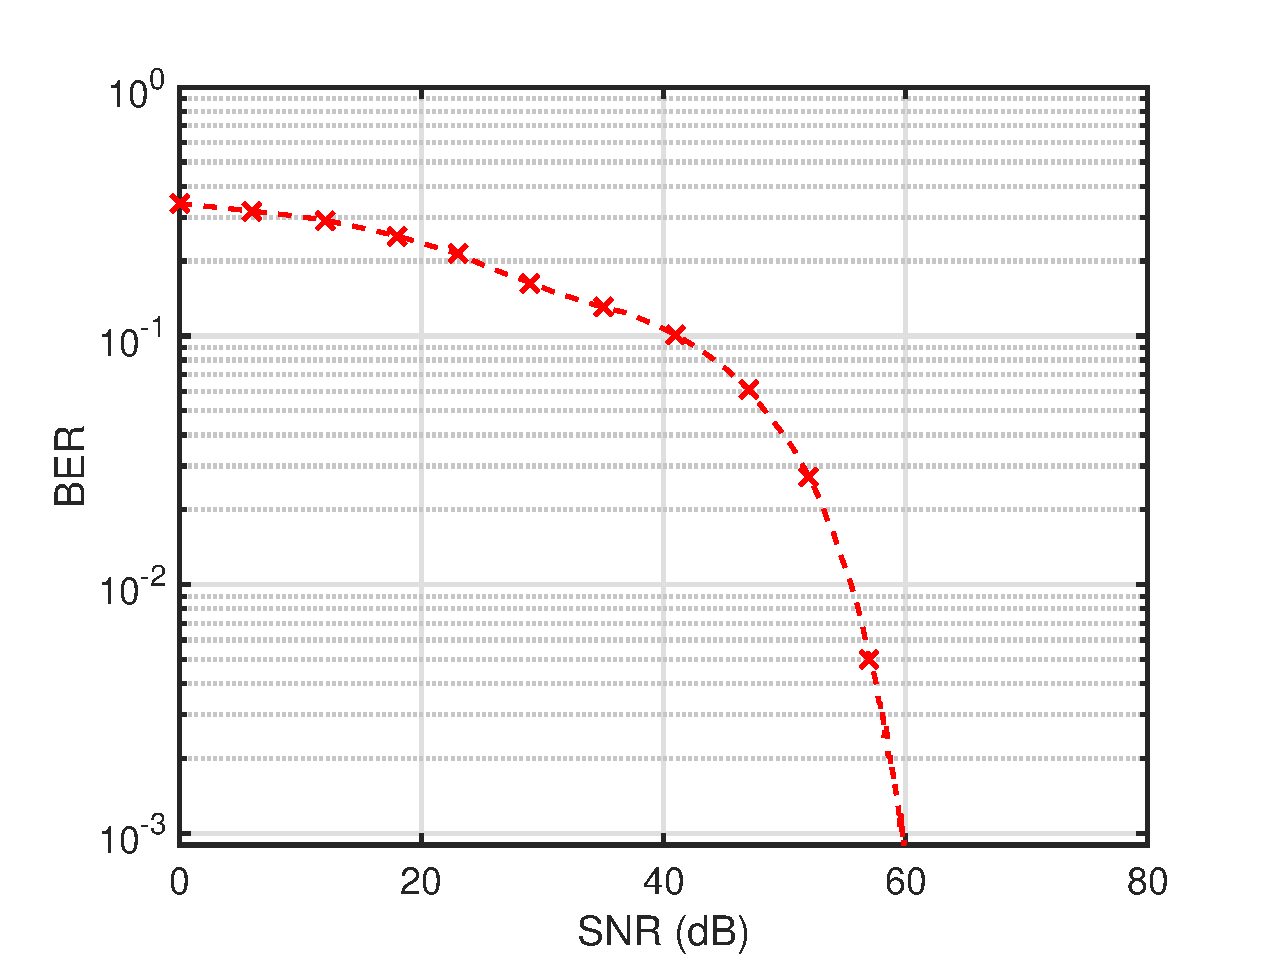
\includegraphics[trim={0.1in 0.0in 0.5in 0.1in}, clip=true, width=0.79\textwidth]{M8_N7_8-MM_BERvsSNR.eps}
			\caption{8-MM, $D$=7}
			\label{fig8MM7}
		\end{subfigure}
	\caption{BER vs SNR for different combinations of CBC}
	\label{figMM_BERvsSNR}
\end{figure}
\clearpage% Flush page
}

\afterpage{%
%\clearpage
\begin{figure}[H]
	\centering
		\begin{subfigure}{\textwidth}
		\centering
			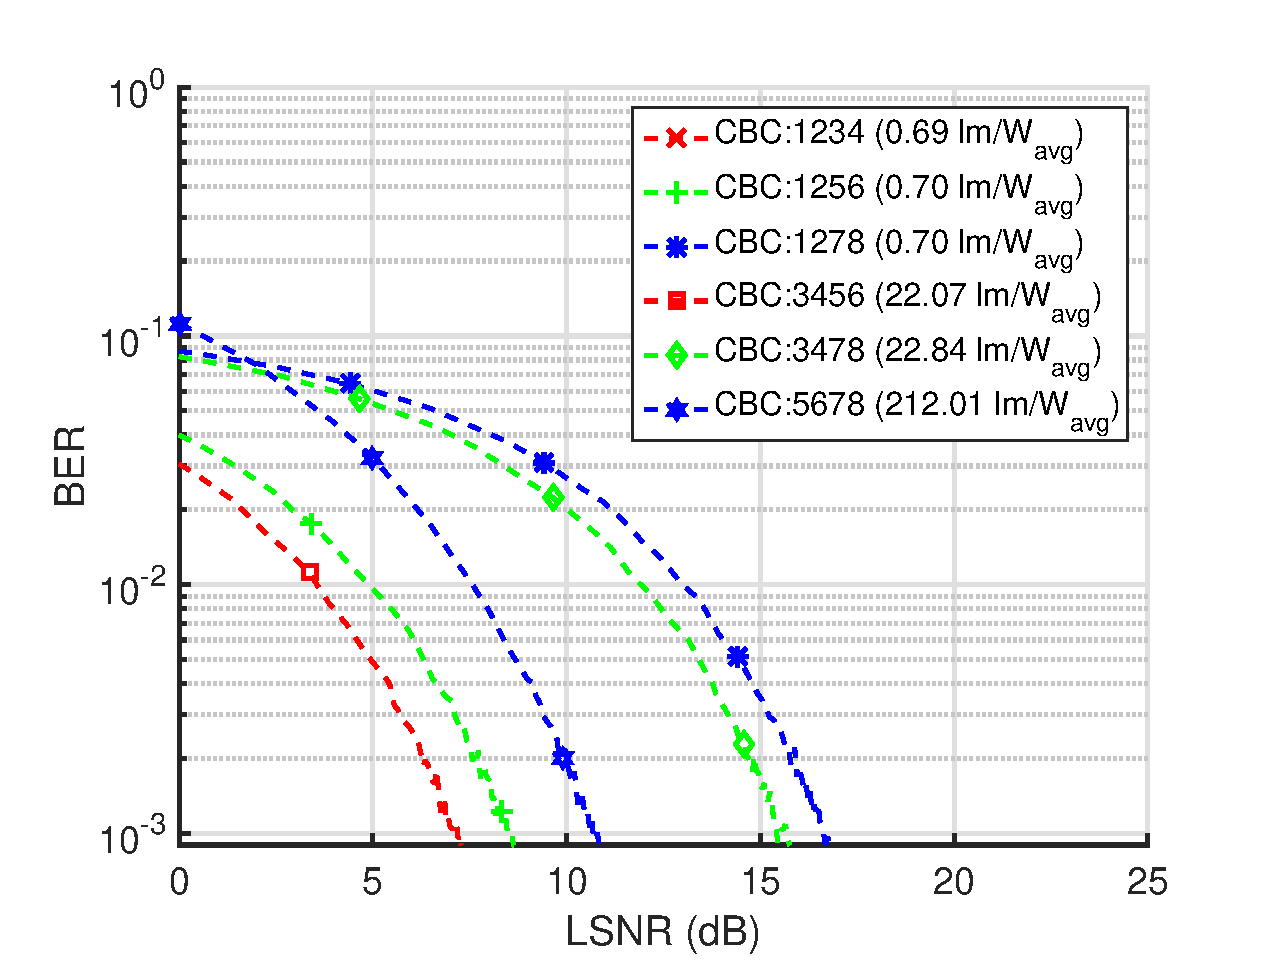
\includegraphics[trim={0.1in 0.0in 0.5in 0.1in}, clip=true, width=0.79\textwidth]{M4_N5_4-MM_BERvsLSNR.eps}
			\caption{4-MM, $D$=5}
			\label{fig4MM5L}
		\end{subfigure}
		%\hfill
		\begin{subfigure}{\textwidth}
		\centering
			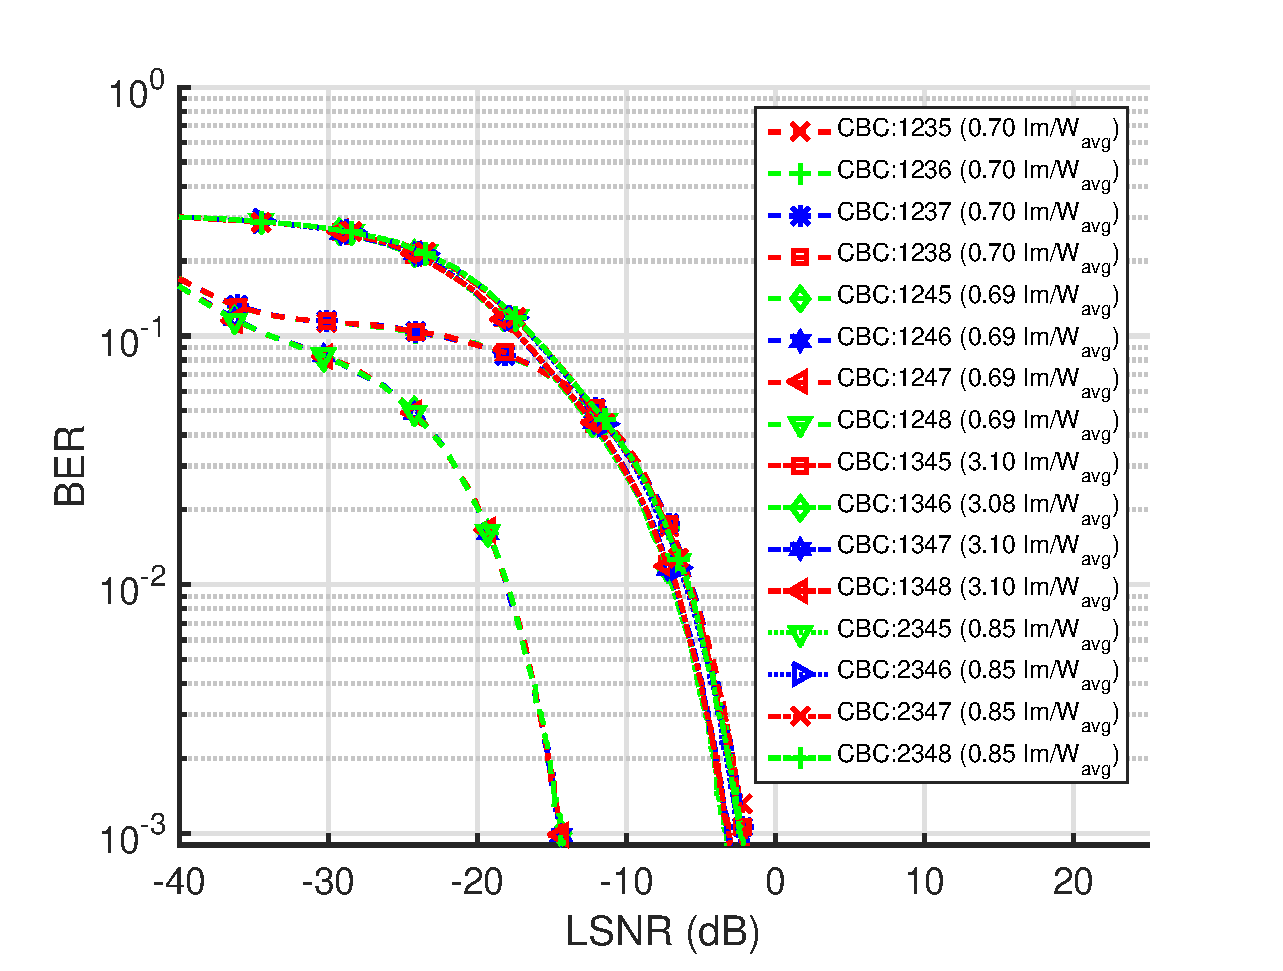
\includegraphics[trim={0.1in 0.0in 0.5in 0.1in}, clip=true, width=0.79\textwidth]{M4_N6_4-MM_BERvsLSNR.eps}
			\caption{4-MM, $D$=6}
			\label{fig4MM6L}
		\end{subfigure}
		%\caption{BER vs LSNR for different combinations of CBC}
	%\label{figMM_BERvsLSNR}
\end{figure}
		%\vfill
\begin{figure}[H]
		\ContinuedFloat
		\begin{subfigure}{\textwidth}
		\centering
			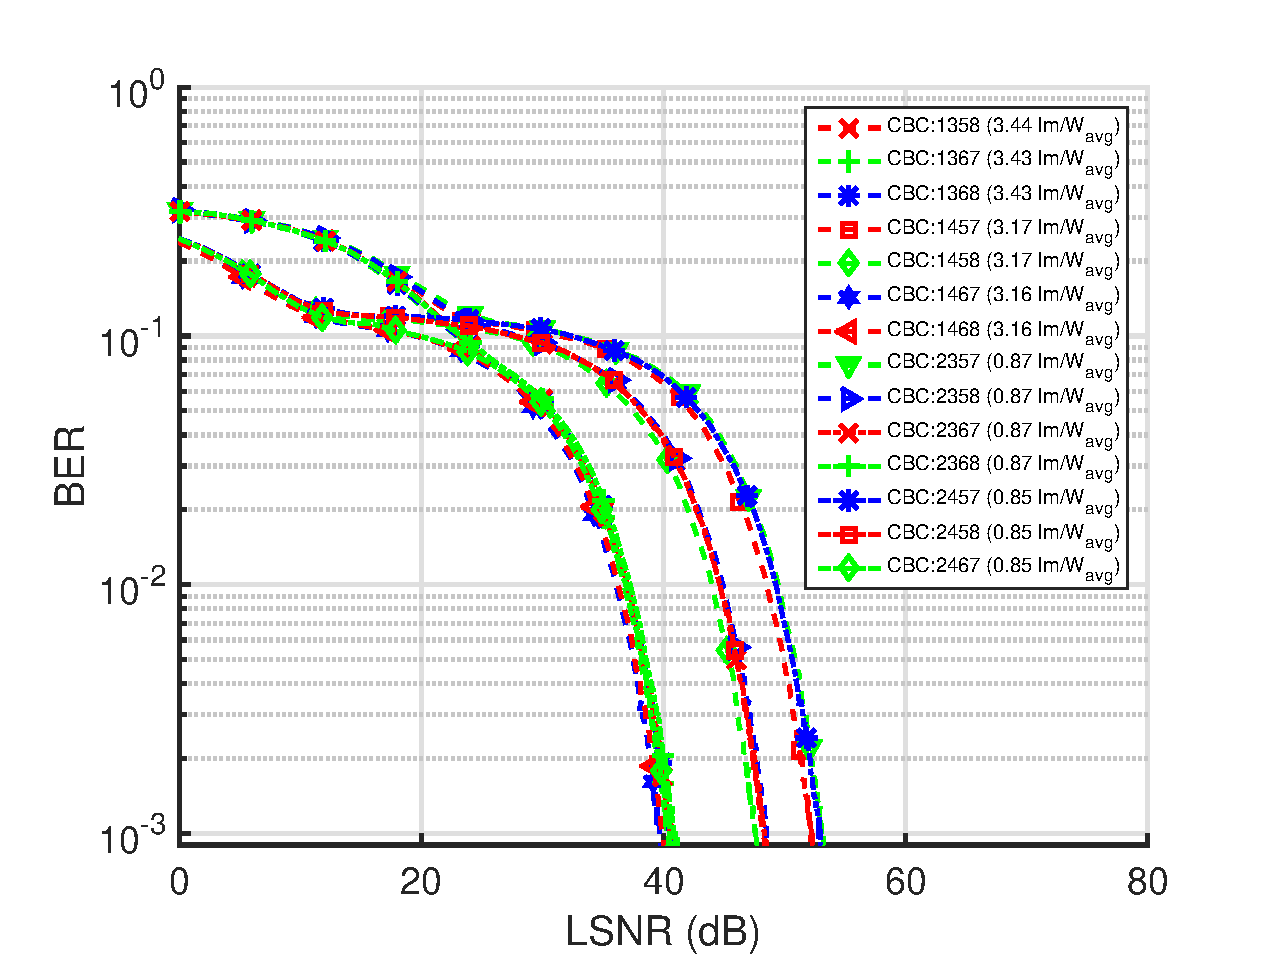
\includegraphics[trim={0.1in 0.0in 0.5in 0.1in}, clip=true, width=0.79\textwidth]{M4_N7_4-MM_BERvsLSNR.eps}
			\caption{4-MM, $D$=7}
			\label{fig4MM7L}
		\end{subfigure}
		%\hfill
		\begin{subfigure}{\textwidth}
		\centering
			\includegraphics[trim={0.1in 0.0in 0.5in 0.1in}, clip=true, width=0.79\textwidth]{4-MM_BERvsLSNR.eps}
			\caption{4-MM}
			\label{fig4MML}
		\end{subfigure}
	\caption{BER vs LSNR for different combinations of CBC}
	\label{figMM_BERvsLSNR}
\end{figure}
\clearpage% Flush page
}

Performance of MM is studied using color bands and color band combinations as defined in the standard and outlined in section \ref{sec:ieeestd}. Each set of LEDs generating a metameric color point can be implemented as a CBC. Block diagram for MM using CBCs is illustrated in \figurename{ \ref{figMMBD}}. For an $M$-ary MM, log$^{ }_{2}$($M$) bits from the encoded bit--stream are mapped to one out of $M$ possible CBCs. With knowledge of color set--point to generate and user requested illumination level, radiant fluxes $P_{d}; 1\leq d\leq D$ to transmit are calculated. The LED drivers then drive all LEDs to achieve desired illumination color and intensity using the CBC selected by the information to transmit. At the receivers, the incident radiant flux generates electrical signals which are used to estimate transmitted flux $\hat{P}_{d}$ over each type of LED. Using the estimated fluxes, an estimate of active set of LEDs $\hat{\text{CBC}}_{m}$ can be made to recover transmitted information.

\figurename{ \ref{figMM_BERvsSNR}} shows BER vs SNR performance for MM for $M$ = 4 and 8. For this analysis, a white chromaticity point of (1/3, 1/3) is generated with the selected CBCs. 4-MM can be implemented with $D$ = 5, 6 or 7. 8-MM is implemented with $D=7$. In absence of illumination constraint, 4-MM achieves the best performance with $D=5$ using CBs from set \{0, 1, 2, 3, 4\} for CBC set \{5, 6, 7, 8\}. Performance plots for 4-MM with $D$ = 6 and 7 are also illustrated for comparison. Implementing 8-MM with CBCs as outlined in IEEE 802.15.7 requires about 60 dB of SNR and seems impractical. However, a different set of LEDs may be used to implement 8-MM to obtain a better performance.

Performance comparison of 4-MM at same illumination intensity level is illustrated in \figurename{ \ref{figMM_BERvsSNR}}. In this case, with $D=5$, 4-MM with CBs from set \{0, 1, 2, 4, 5\} for CBC set \{3, 4, 5, 6\} outperforms others.  CBC set \{5, 6, 7, 8\} has a high luminous efficacy as compared to  CBC set \{3, 4, 5, 6\} and thus is constrained in radiant flux for signaling at a set illumination level. On comparing performance of 4-MM for all possible values of $D$, CBC sets \{1, 2, 4, 5\}, \{1, 2, 4, 6\}, \{1, 2, 4, 7\} and \{1, 2, 4, 8\} with $D=6$ perform the best.